\originalchapter{8.322公开作业一至七：辐射与自洽场}
以下题面按2003年实际作业中文重述；全部答案为自主推导，不是取得的官方解答。只给商书编号的题逐项留到末表，不能靠熟悉Sakurai补出题面。作业2、5均只有此类引用，故没有另造整章“答案”。

\originalsection{PS1 Q5：任意自旋的旋转磁场}
\begin{exercise}
初态$J^2=j(j+1)\hbar^2,J_z=j\hbar$。$t>0$施加$\vct B=B_0\hat z+B_1(\hat x\cos\omega t+\hat y\sin\omega t)$，$H=-\alpha\vct J\cdot\vct B$。(a)给出任意$t$的精确态；(b)写共振时的经典$\vct J(t)$；(c)在$\langle J_z\rangle=0$的时刻比较经典与量子。原(b)印“$\omega=\alpha$”，与给定Hamiltonian的单位/符号不一致，应由实际共振条件解释。
\end{exercise}
\begin{solution}
设$\Delta=\alpha B_0+\omega$、$\Omega=\sqrt{\Delta^2+(\alpha B_1)^2}$。旋转系给$U=e^{-i\omega tJ_z/\hbar}e^{it(\alpha B_1J_x+\Delta J_z)/\hbar}$。自旋$j$最高权态是$2j$个自旋$1/2$的完全对称积；定义
\[
 a=e^{-i\omega t/2}[\cos(\Omega t/2)+i(\Delta/\Omega)\sin(\Omega t/2)],\quad
 b=ie^{i\omega t/2}(\alpha B_1/\Omega)\sin(\Omega t/2),
\]
则$|\psi(t)\rangle=\sum_{m=-j}^j\sqrt{\binom{2j}{j-m}}a^{j+m}b^{j-m}|j,m\rangle$，归一由$|a|^2+|b|^2=1$和二项式保证。

共振本约定为$\omega=-\alpha B_0$。经典方程$\dot{\vct J}=\alpha\vct J\times\vct B$在旋转系变成绕$x$的匀速进动，返回实验室得
\[
 \vct J(t)=j\hbar(-\sin\alpha B_1t\sin\omega t,
 \sin\alpha B_1t\cos\omega t,\cos\alpha B_1t).
\]
量子平均完全相同，因为线性自旋Hamiltonian封闭Ehrenfest方程。首次零$z$均值时$|\alpha B_1|t=\pi/2$，量子$J_z$分布为$\binom{2j}{j-m}2^{-2j}$，方差$j\hbar^2/2$，并非经典确定读数0；沿平均方向仍是最大权自旋相干态。相对平均长度的涨落$1/\sqrt{2j}$在大$j$变小。没有将原印的无量纲共振条件硬套到有单位的$B_0$。
\end{solution}

\originalsection{PS3 Q1、Q3：态密度与所有超精细分支}
\begin{exercise}
Q1：用课堂盒归一求能量$E=\hbar\omega$、固定偏振、立体角$\dd\Omega$内光子的态密度，类比课堂电子态密度。Q3：(a)忽略核自旋，求氢$2\,{}^2P_{1/2},m_j=1/2$衰变到$1\,{}^2S_{1/2},m_j=\pm1/2$的速率；(b)对氘$I=1$，求所有$F,m_F\to F',m'_F$超精细分支。Q3虽提到未附书题Q2，所需原子态和实际任务均完整给出，以下从头计算基础总速率。
\end{exercise}
\begin{solution}
盒中每偏振每态占$\vct k$体积$(2\pi)^3/V$。$\dd N=Vk^2\dd k\dd\Omega/(2\pi)^3$、$E=\hbar ck$，故$\rho_\gamma(E)\dd\Omega=VE^2\dd\Omega/[(2\pi)^3\hbar^3c^3]$，不额外乘2。电子为$Vp^2\dd p\dd\Omega/(2\pi\hbar)^3$、$\dd E=(p/m)\dd p$，给$Vm p\dd\Omega/(2\pi\hbar)^3$；若总自旋数另算，须说明。

径向函数$R_{10}=2a_0^{-3/2}e^{-r/a_0}$、$R_{21}=r e^{-r/(2a_0)}/(2\sqrt6a_0^{5/2})$。径向偶极积分
\[
 D_r=\int_0^\infty R_{10}R_{21}r^3\dd r
 =\frac{256}{81\sqrt6}a_0.
\]
每个初$2p$磁态的总偶极强度为$e^2D_r^2/3$，故定义$\Gamma_0(\omega)=e^2\omega^3D_r^2/(9\pi\epsilon_0\hbar c^3)$。非相对论跃迁频率给约$6.27\times10^8\,\mathrm{s}^{-1}$。初$j=1/2,m=1/2$为$-\sqrt{1/3}|m_l=0,\uparrow\rangle+\sqrt{2/3}|m_l=1,\downarrow\rangle$，电偶极不翻自旋，两个末态速率分别$\Gamma_0/3,2\Gamma_0/3$。

氘的$F,F'=1/2,3/2$。选球分量$q=m'-m$，Wigner--Eckart给每一分支系数
\[
 b_{Fm,F'm'}=2(2F+1)(2F'+1)
 \begin{Bmatrix}\tfrac12&F'&1\\F&\tfrac12&1\end{Bmatrix}^{\!2}
 \begin{pmatrix}F'&1&F\\-m'&m'-m&m\end{pmatrix}^{\!2},\quad
 \Gamma_{Fm\to F'm'}=b_{Fm,F'm'}\Gamma_0(\omega_{FF'}).
\]
不满足$|m'-m|\le1$的项为0。为给出所有实际分支，行列顺序均取
\[\begin{gathered}(1/2,1/2),(1/2,-1/2),(3/2,3/2),\\(3/2,1/2),(3/2,-1/2),(3/2,-3/2).\end{gathered}\]
系数矩阵为
\[
 b=\frac1{27}\begin{pmatrix}
 1&2&12&8&4&0\\2&1&0&4&8&12\\
 12&0&9&6&0&0\\8&4&6&1&8&0\\
 4&8&0&8&1&6\\0&12&0&0&6&9
 \end{pmatrix}.
\]
每行和1，故忽略微小超精细频率差时总寿命一致。若保留各$\omega_{FF'}^3$，须用相应初末超精细能差，不能仍将精确总和称$\Gamma_0$。氘约化质量将$a_0$和基准频率一致替换，不影响角系数。
\end{solution}

\originalsection{PS3 Q4、Q5：被E1禁止的跃迁}
\begin{exercise}
Q4：求自由空间氢$2\,{}^2S_{1/2},F=1\to2\,{}^2S_{1/2},F=0$单光子超精细衰变率。Q5：求氢$3d\to1s$单光子衰变率。均须说明多极类型。
\end{exercise}
\begin{solution}
Q4同为$2S$，宇称相同且轨道径向不变，E1为0。M1磁矩为$-g_e\mu_B\vct S/\hbar+g_p\mu_N\vct I/\hbar$，$F=1,m=0$至单态的$z$矩元为$-(g_e\mu_B+g_p\mu_N)/2$；另两$m$经球分量有相同总强度。故
\[
 \Gamma=\frac{\mu_0\omega_{2S}^3}{3\pi\hbar c^3}
 \left(\frac{g_e\mu_B+g_p\mu_N}{2}\right)^2.
\]
用非相对论Fermi接触项，$\hbar\omega_{nS}=(2\mu_0/3)g_e\mu_Bg_p\mu_N|\psi_{nS}(0)|^2$，$|\psi_{2S}(0)|^2=1/(8\pi a_0^3)$，得到约$5.6\times10^{-18}\,\mathrm{s}^{-1}$；这是领先阶模型，未含QED/核结构。\textbf{原题是$2S$，不是$1S$的21厘米线}，不能将后者$\omega$直接代入。实际$2S$还经两光子$2S\to1S$快速衰变；本题所问仅这个极弱单光子通道。

Q5宇称同、$\Delta l=2$，最低允许E2。$R_{32}=4r^2e^{-r/(3a_0)}/(81\sqrt{30}a_0^{7/2})$给
\[
 Q_r=\int R_{10}R_{32}r^4\dd r
 =\frac{1215}{128\sqrt{30}}a_0^2.
\]
初$m=0$时$\langle r_z^2\rangle_{fi}=2Q_r/(3\sqrt5)$、$\langle r_x^2\rangle=\langle r_y^2\rangle=-Q_r/(3\sqrt5)$，其迹为0。$Q_{ij}=-3e\langle r_ir_j\rangle$给$\sum|Q_{ij}|^2=6e^2Q_r^2/5$；旋转对称保证其他$m$同速率。代入上章系数，
\[
 \Gamma_{3d\to1s}=\frac{e^2\omega^5Q_r^2}{300\pi\epsilon_0\hbar c^5}
 \simeq5.94\times10^2\,\mathrm{s}^{-1},\qquad
 \hbar\omega={\rm Ry}\,(1-1/9).
\]
这里只计单光子到$1s$，$3d\to2p$的E1通道另存在，不能用此率的倒数当总寿命。
\end{solution}

\originalsection{PS4 Q2、Q3：自旋的绝热相位}
\begin{exercise}
自旋$s$，$\vct B(t)=B(\sin\theta\cos\phi(t),\sin\theta\sin\phi(t),\cos\theta)$，$H=2\vct B\cdot\vct J/\hbar$。初$|m,t=0\rangle$。(Q2)求绝热态$e^{i\alpha_m(t)}|m,t\rangle$的相位；(Q3)方向绕$z$完整一周求Berry相位并比较前题。原Q3印“比较problem 3”，按相邻Q2解释并保留更正记录。
\end{exercise}
\begin{solution}
这里$B$因原Hamiltonian定义有能量单位；$E_m=2Bm$。选$|m,t\rangle=e^{-i\phi(t)J_z/\hbar}e^{-i\theta J_y/\hbar}|m\rangle$，直接微分给$i\langle m,t|\dot m,t\rangle=m\cos\theta\dot\phi$。因而$\alpha_m=-2Bmt/\hbar+m\cos\theta[\phi(t)-\phi(0)]$。这个连续规范绕一周的末矢量还有$e^{-i2\pi m}$，闭环物理几何相位合计
$\gamma_m=2\pi m(\cos\theta-1)=-m\Omega\pmod{2\pi}$，$\Omega=2\pi(1-\cos\theta)$。半整数态不能忘掉这一下标架回转符号。绝热条件对相邻能级用上章能隙判据，典型为$\hbar|\dot\phi|\sin\theta\ll2B$；没有非零能隙时本推导不适用。
\end{solution}

\originalsection{PS6 Q3、Q4：偶数简并与完整能带}
\begin{exercise}
Q3：$\Theta^2=-1$且Hamiltonian时间反演不变，证明不可能有三重能级。Q4：Kronig--Penney势$V(x)=\lambda\sum_n\delta(x-na)$，$\hbar=m=1$，分析能带；在$0\le\lambda,\sqrt{2E}\le100$内画允许区，分析固定$\lambda$的大$E$和固定$E$的大$\lambda$。
\end{exercise}
\begin{solution}
有限维某能级空间在$\Theta$下不变。反幺正内积恒等式结合$\Theta^2=-1$给$\langle u|\Theta u\rangle=0$。选一个归一$u$，$\operatorname{span}(u,\Theta u)$的正交补也在$\Theta$下不变（分别用反幺正内积验证）。重复配对直至耗尽，维数为偶数，三重不可能。只证明至少两态还不足排除三重，故需要这一步正交补归纳。

设$q=\sqrt{2E}$。自由单胞矩阵$P=\left(\begin{smallmatrix}\cos qa&\sin qa/q\\-q\sin qa&\cos qa\end{smallmatrix}\right)$，delta跨越$\psi'(0^+)-\psi'(0^-)=2\lambda\psi(0)$给$D=\left(\begin{smallmatrix}1&0\\2\lambda&1\end{smallmatrix}\right)$。$\det DP=1$，迹给精确色散
\[
 \cos Ka=\cos qa+\frac\lambda q\sin qa,\qquad
 \left|\cos qa+\frac\lambda q\sin qa\right|\le1.
\]
原题未指定$a$，图明确取$a=1$；一般图用$qa,\lambda a$缩放，能量单位为$a^{-2}$。固定$\lambda$且$q\to\infty$时修正$O(\lambda/q)$，波数禁带宽缩小，远离Bragg点趋自由；能量禁带宽却可保持有限，不能说所有能隙绝对趋0。固定有限$q$且$\lambda\to\infty$，除$qa=n\pi$及其越来越窄邻域皆禁，极限是单独Dirichlet阱$E_n=n^2\pi^2/(2a^2)$；不是所有有限$E$都允许。蓝区边界逐带求精确根，显示如下完整范围。
\begin{figure}[htbp]\centering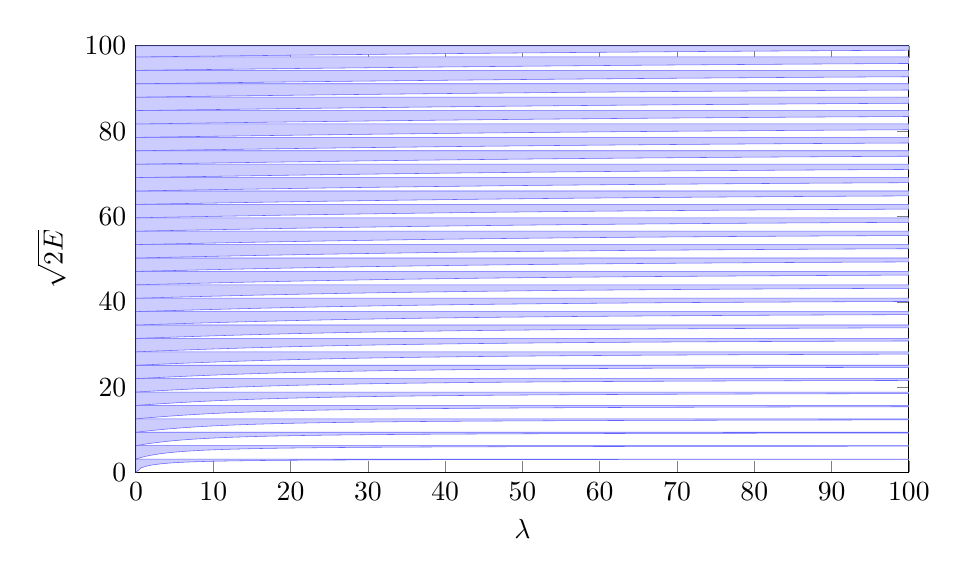
\begin{tikzpicture}\begin{axis}[width=.94\textwidth,height=7cm,xlabel={$\lambda$},ylabel={$\sqrt{2E}$},xmin=0,xmax=100,ymin=0,ymax=100]
\addplot[draw=blue!60,fill=blue!20,line width=.2pt] coordinates {(0,0) (0.66667,1.094322) (1.3333,1.47201) (2,1.720667) (2.6667,1.902311) (3.3333,2.042228) (4,2.153748) (4.6667,2.24486) (5.3333,2.320739) (6,2.384918) (6.6667,2.439904) (7.3333,2.487534) (8,2.529183) (8.6667,2.565905) (9.3333,2.59852) (10,2.627675) (10.667,2.653891) (11.333,2.677586) (12,2.699106) (12.667,2.718734) (13.333,2.736709) (14,2.75323) (14.667,2.768465) (15.333,2.782558) (16,2.795631) (16.667,2.807792) (17.333,2.819132) (18,2.829731) (18.667,2.839658) (19.333,2.848977) (20,2.85774) (20.667,2.865996) (21.333,2.873787) (22,2.881152) (22.667,2.888124) (23.333,2.894734) (24,2.901009) (24.667,2.906974) (25.333,2.912652) (26,2.918062) (26.667,2.923223) (27.333,2.928152) (28,2.932864) (28.667,2.937372) (29.333,2.941691) (30,2.945831) (30.667,2.949804) (31.333,2.953619) (32,2.957286) (32.667,2.960812) (33.333,2.964207) (34,2.967476) (34.667,2.970628) (35.333,2.973668) (36,2.976601) (36.667,2.979434) (37.333,2.982172) (38,2.984819) (38.667,2.987379) (39.333,2.989858) (40,2.992258) (40.667,2.994583) (41.333,2.996838) (42,2.999024) (42.667,3.001145) (43.333,3.003204) (44,3.005204) (44.667,3.007147) (45.333,3.009036) (46,3.010872) (46.667,3.012658) (47.333,3.014396) (48,3.016087) (48.667,3.017735) (49.333,3.019339) (50,3.020903) (50.667,3.022428) (51.333,3.023914) (52,3.025364) (52.667,3.026778) (53.333,3.028158) (54,3.029506) (54.667,3.030822) (55.333,3.032108) (56,3.033364) (56.667,3.034592) (57.333,3.035792) (58,3.036965) (58.667,3.038113) (59.333,3.039236) (60,3.040335) (60.667,3.04141) (61.333,3.042463) (62,3.043494) (62.667,3.044504) (63.333,3.045493) (64,3.046463) (64.667,3.047412) (65.333,3.048344) (66,3.049257) (66.667,3.050152) (67.333,3.05103) (68,3.051891) (68.667,3.052737) (69.333,3.053566) (70,3.05438) (70.667,3.055179) (71.333,3.055964) (72,3.056734) (72.667,3.057491) (73.333,3.058235) (74,3.058965) (74.667,3.059683) (75.333,3.060388) (76,3.061081) (76.667,3.061763) (77.333,3.062433) (78,3.063092) (78.667,3.06374) (79.333,3.064378) (80,3.065005) (80.667,3.065622) (81.333,3.066229) (82,3.066827) (82.667,3.067415) (83.333,3.067994) (84,3.068564) (84.667,3.069125) (85.333,3.069678) (86,3.070222) (86.667,3.070759) (87.333,3.071287) (88,3.071807) (88.667,3.07232) (89.333,3.072825) (90,3.073323) (90.667,3.073814) (91.333,3.074298) (92,3.074775) (92.667,3.075245) (93.333,3.075708) (94,3.076166) (94.667,3.076617) (95.333,3.077061) (96,3.0775) (96.667,3.077933) (97.333,3.07836) (98,3.078781) (98.667,3.079197) (99.333,3.079607) (100,3.080012) (100,3.141593) (0,3.141593)} --cycle;
\addplot[draw=blue!60,fill=blue!20,line width=.2pt] coordinates {(0,3.141593) (0.66667,3.516328) (1.3333,3.814181) (2,4.057516) (2.6667,4.260163) (3.3333,4.431415) (4,4.577859) (4.6667,4.704347) (5.3333,4.814546) (6,4.911288) (6.6667,4.996798) (7.3333,5.072848) (8,5.140863) (8.6667,5.202006) (9.3333,5.25723) (10,5.307325) (10.667,5.35295) (11.333,5.394659) (12,5.432919) (12.667,5.468131) (13.333,5.500633) (14,5.530719) (14.667,5.558642) (15.333,5.584622) (16,5.60885) (16.667,5.631494) (17.333,5.652701) (18,5.672601) (18.667,5.691309) (19.333,5.708926) (20,5.725545) (20.667,5.741246) (21.333,5.756102) (22,5.770179) (22.667,5.783535) (23.333,5.796223) (24,5.808292) (24.667,5.819785) (25.333,5.830743) (26,5.841201) (26.667,5.851192) (27.333,5.860747) (28,5.869892) (28.667,5.878655) (29.333,5.887058) (30,5.895122) (30.667,5.902867) (31.333,5.910312) (32,5.917474) (32.667,5.924369) (33.333,5.93101) (34,5.937412) (34.667,5.943588) (35.333,5.949548) (36,5.955304) (36.667,5.960867) (37.333,5.966245) (38,5.971448) (38.667,5.976484) (39.333,5.981361) (40,5.986086) (40.667,5.990666) (41.333,5.995108) (42,5.999418) (42.667,6.003602) (43.333,6.007665) (44,6.011612) (44.667,6.015448) (45.333,6.019178) (46,6.022805) (46.667,6.026335) (47.333,6.029771) (48,6.033117) (48.667,6.036376) (49.333,6.039551) (50,6.042646) (50.667,6.045664) (51.333,6.048607) (52,6.051478) (52.667,6.054281) (53.333,6.057016) (54,6.059687) (54.667,6.062297) (55.333,6.064846) (56,6.067337) (56.667,6.069772) (57.333,6.072153) (58,6.074481) (58.667,6.076759) (59.333,6.078988) (60,6.08117) (60.667,6.083305) (61.333,6.085396) (62,6.087444) (62.667,6.089449) (63.333,6.091415) (64,6.093341) (64.667,6.095228) (65.333,6.097079) (66,6.098894) (66.667,6.100673) (67.333,6.102419) (68,6.104132) (68.667,6.105813) (69.333,6.107462) (70,6.109081) (70.667,6.110671) (71.333,6.112232) (72,6.113765) (72.667,6.115271) (73.333,6.11675) (74,6.118204) (74.667,6.119632) (75.333,6.121036) (76,6.122416) (76.667,6.123773) (77.333,6.125107) (78,6.126419) (78.667,6.12771) (79.333,6.12898) (80,6.130229) (80.667,6.131457) (81.333,6.132667) (82,6.133857) (82.667,6.135029) (83.333,6.136182) (84,6.137318) (84.667,6.138436) (85.333,6.139537) (86,6.140622) (86.667,6.141691) (87.333,6.142743) (88,6.14378) (88.667,6.144802) (89.333,6.145809) (90,6.146802) (90.667,6.14778) (91.333,6.148744) (92,6.149695) (92.667,6.150632) (93.333,6.151557) (94,6.152468) (94.667,6.153367) (95.333,6.154254) (96,6.155129) (96.667,6.155992) (97.333,6.156843) (98,6.157683) (98.667,6.158512) (99.333,6.159331) (100,6.160138) (100,6.283185) (0,6.283185)} --cycle;
\addplot[draw=blue!60,fill=blue!20,line width=.2pt] coordinates {(0,6.283185) (0.66667,6.487975) (1.3333,6.67736) (2,6.851237) (2.6667,7.010177) (3.3333,7.155125) (4,7.287194) (4.6667,7.407542) (5.3333,7.517298) (6,7.617524) (6.6667,7.709196) (7.3333,7.793198) (8,7.870323) (8.6667,7.94128) (9.3333,8.006698) (10,8.067136) (10.667,8.123087) (11.333,8.174991) (12,8.223235) (12.667,8.268166) (13.333,8.310089) (14,8.349276) (14.667,8.38597) (15.333,8.420388) (16,8.452724) (16.667,8.483152) (17.333,8.511827) (18,8.538889) (18.667,8.564465) (19.333,8.588668) (20,8.611603) (20.667,8.633362) (21.333,8.65403) (22,8.673684) (22.667,8.692395) (23.333,8.710227) (24,8.727238) (24.667,8.743483) (25.333,8.75901) (26,8.773865) (26.667,8.788089) (27.333,8.80172) (28,8.814795) (28.667,8.827345) (29.333,8.839401) (30,8.850991) (30.667,8.86214) (31.333,8.872874) (32,8.883214) (32.667,8.893181) (33.333,8.902794) (34,8.912073) (34.667,8.921033) (35.333,8.929691) (36,8.938061) (36.667,8.946157) (37.333,8.953992) (38,8.961579) (38.667,8.968929) (39.333,8.976053) (40,8.98296) (40.667,8.989661) (41.333,8.996164) (42,9.002478) (42.667,9.008612) (43.333,9.014571) (44,9.020365) (44.667,9.025999) (45.333,9.03148) (46,9.036814) (46.667,9.042006) (47.333,9.047063) (48,9.05199) (48.667,9.056791) (49.333,9.061471) (50,9.066034) (50.667,9.070486) (51.333,9.074829) (52,9.079068) (52.667,9.083206) (53.333,9.087248) (54,9.091195) (54.667,9.095052) (55.333,9.098822) (56,9.102507) (56.667,9.10611) (57.333,9.109634) (58,9.113082) (58.667,9.116456) (59.333,9.119757) (60,9.12299) (60.667,9.126155) (61.333,9.129255) (62,9.132291) (62.667,9.135266) (63.333,9.138182) (64,9.14104) (64.667,9.143841) (65.333,9.146588) (66,9.149283) (66.667,9.151926) (67.333,9.154519) (68,9.157063) (68.667,9.15956) (69.333,9.162012) (70,9.164418) (70.667,9.166781) (71.333,9.169102) (72,9.171382) (72.667,9.173622) (73.333,9.175822) (74,9.177985) (74.667,9.18011) (75.333,9.182199) (76,9.184253) (76.667,9.186273) (77.333,9.188259) (78,9.190213) (78.667,9.192135) (79.333,9.194025) (80,9.195885) (80.667,9.197716) (81.333,9.199518) (82,9.201291) (82.667,9.203037) (83.333,9.204756) (84,9.206448) (84.667,9.208115) (85.333,9.209757) (86,9.211374) (86.667,9.212967) (87.333,9.214536) (88,9.216082) (88.667,9.217606) (89.333,9.219108) (90,9.220588) (90.667,9.222048) (91.333,9.223486) (92,9.224905) (92.667,9.226303) (93.333,9.227682) (94,9.229043) (94.667,9.230384) (95.333,9.231708) (96,9.233013) (96.667,9.234301) (97.333,9.235572) (98,9.236827) (98.667,9.238064) (99.333,9.239286) (100,9.240491) (100,9.424778) (0,9.424778)} --cycle;
\addplot[draw=blue!60,fill=blue!20,line width=.2pt] coordinates {(0,9.424778) (0.66667,9.563965) (1.3333,9.698035) (2,9.826361) (2.6667,9.948557) (3.3333,10.06444) (4,10.17397) (4.6667,10.27726) (5.3333,10.37448) (6,10.46588) (6.6667,10.55174) (7.3333,10.63236) (8,10.70806) (8.6667,10.77915) (9.3333,10.84594) (10,10.90871) (10.667,10.96774) (11.333,11.02331) (12,11.07565) (12.667,11.12499) (13.333,11.17156) (14,11.21554) (14.667,11.25712) (15.333,11.29647) (16,11.33374) (16.667,11.36909) (17.333,11.40263) (18,11.4345) (18.667,11.4648) (19.333,11.49364) (20,11.52112) (20.667,11.54731) (21.333,11.57231) (22,11.59619) (22.667,11.61901) (23.333,11.64085) (24,11.66175) (24.667,11.68178) (25.333,11.70099) (26,11.71942) (26.667,11.73712) (27.333,11.75413) (28,11.77048) (28.667,11.78621) (29.333,11.80136) (30,11.81596) (30.667,11.83003) (31.333,11.8436) (32,11.85669) (32.667,11.86934) (33.333,11.88156) (34,11.89337) (34.667,11.90479) (35.333,11.91584) (36,11.92654) (36.667,11.93691) (37.333,11.94695) (38,11.95669) (38.667,11.96613) (39.333,11.97529) (40,11.98418) (40.667,11.99282) (41.333,12.00121) (42,12.00936) (42.667,12.01728) (43.333,12.02499) (44,12.03249) (44.667,12.03979) (45.333,12.0469) (46,12.05382) (46.667,12.06056) (47.333,12.06713) (48,12.07353) (48.667,12.07978) (49.333,12.08587) (50,12.09181) (50.667,12.09761) (51.333,12.10327) (52,12.1088) (52.667,12.1142) (53.333,12.11948) (54,12.12464) (54.667,12.12968) (55.333,12.13461) (56,12.13943) (56.667,12.14414) (57.333,12.14875) (58,12.15327) (58.667,12.15769) (59.333,12.16202) (60,12.16625) (60.667,12.1704) (61.333,12.17447) (62,12.17846) (62.667,12.18236) (63.333,12.18619) (64,12.18994) (64.667,12.19362) (65.333,12.19724) (66,12.20078) (66.667,12.20425) (67.333,12.20766) (68,12.21101) (68.667,12.2143) (69.333,12.21752) (70,12.22069) (70.667,12.2238) (71.333,12.22686) (72,12.22986) (72.667,12.23282) (73.333,12.23572) (74,12.23857) (74.667,12.24137) (75.333,12.24412) (76,12.24683) (76.667,12.2495) (77.333,12.25212) (78,12.2547) (78.667,12.25723) (79.333,12.25973) (80,12.26218) (80.667,12.2646) (81.333,12.26698) (82,12.26932) (82.667,12.27163) (83.333,12.2739) (84,12.27614) (84.667,12.27834) (85.333,12.28051) (86,12.28265) (86.667,12.28475) (87.333,12.28683) (88,12.28887) (88.667,12.29089) (89.333,12.29287) (90,12.29483) (90.667,12.29676) (91.333,12.29867) (92,12.30054) (92.667,12.30239) (93.333,12.30422) (94,12.30602) (94.667,12.3078) (95.333,12.30955) (96,12.31128) (96.667,12.31298) (97.333,12.31467) (98,12.31633) (98.667,12.31797) (99.333,12.31959) (100,12.32118) (100,12.56637) (0,12.56637)} --cycle;
\addplot[draw=blue!60,fill=blue!20,line width=.2pt] coordinates {(0,12.56637) (0.66667,12.6715) (1.3333,12.77437) (2,12.8746) (2.6667,12.97187) (3.3333,13.06595) (4,13.15667) (4.6667,13.24393) (5.3333,13.32768) (6,13.40791) (6.6667,13.48467) (7.3333,13.55801) (8,13.62802) (8.6667,13.69481) (9.3333,13.75849) (10,13.81919) (10.667,13.87704) (11.333,13.93217) (12,13.9847) (12.667,14.03478) (13.333,14.08253) (14,14.12806) (14.667,14.1715) (15.333,14.21297) (16,14.25256) (16.667,14.29039) (17.333,14.32654) (18,14.36112) (18.667,14.3942) (19.333,14.42588) (20,14.45622) (20.667,14.4853) (21.333,14.51319) (22,14.53995) (22.667,14.56565) (23.333,14.59033) (24,14.61406) (24.667,14.63688) (25.333,14.65883) (26,14.67997) (26.667,14.70034) (27.333,14.71997) (28,14.73889) (28.667,14.75715) (29.333,14.77478) (30,14.7918) (30.667,14.80825) (31.333,14.82415) (32,14.83953) (32.667,14.85441) (33.333,14.86881) (34,14.88276) (34.667,14.89627) (35.333,14.90937) (36,14.92207) (36.667,14.93439) (37.333,14.94635) (38,14.95796) (38.667,14.96923) (39.333,14.98018) (40,14.99082) (40.667,15.00117) (41.333,15.01124) (42,15.02103) (42.667,15.03056) (43.333,15.03983) (44,15.04887) (44.667,15.05767) (45.333,15.06624) (46,15.0746) (46.667,15.08275) (47.333,15.0907) (48,15.09846) (48.667,15.10603) (49.333,15.11341) (50,15.12063) (50.667,15.12767) (51.333,15.13455) (52,15.14128) (52.667,15.14785) (53.333,15.15427) (54,15.16055) (54.667,15.1667) (55.333,15.17271) (56,15.17859) (56.667,15.18435) (57.333,15.18998) (58,15.1955) (58.667,15.2009) (59.333,15.20619) (60,15.21138) (60.667,15.21646) (61.333,15.22144) (62,15.22632) (62.667,15.23111) (63.333,15.2358) (64,15.24041) (64.667,15.24493) (65.333,15.24936) (66,15.25371) (66.667,15.25797) (67.333,15.26216) (68,15.26628) (68.667,15.27032) (69.333,15.27429) (70,15.27818) (70.667,15.28201) (71.333,15.28577) (72,15.28947) (72.667,15.29311) (73.333,15.29668) (74,15.30019) (74.667,15.30364) (75.333,15.30704) (76,15.31038) (76.667,15.31367) (77.333,15.3169) (78,15.32008) (78.667,15.32321) (79.333,15.32629) (80,15.32932) (80.667,15.3323) (81.333,15.33524) (82,15.33814) (82.667,15.34099) (83.333,15.34379) (84,15.34655) (84.667,15.34928) (85.333,15.35196) (86,15.3546) (86.667,15.35721) (87.333,15.35977) (88,15.3623) (88.667,15.3648) (89.333,15.36725) (90,15.36968) (90.667,15.37207) (91.333,15.37442) (92,15.37675) (92.667,15.37904) (93.333,15.3813) (94,15.38353) (94.667,15.38573) (95.333,15.3879) (96,15.39004) (96.667,15.39216) (97.333,15.39424) (98,15.3963) (98.667,15.39833) (99.333,15.40034) (100,15.40232) (100,15.70796) (0,15.70796)} --cycle;
\addplot[draw=blue!60,fill=blue!20,line width=.2pt] coordinates {(0,15.70796) (0.66667,15.79234) (1.3333,15.87554) (2,15.95733) (2.6667,16.0375) (3.3333,16.11588) (4,16.19233) (4.6667,16.26673) (5.3333,16.33899) (6,16.40906) (6.6667,16.47691) (7.3333,16.5425) (8,16.60586) (8.6667,16.66699) (9.3333,16.72592) (10,16.78269) (10.667,16.83736) (11.333,16.88997) (12,16.94059) (12.667,16.98928) (13.333,17.03611) (14,17.08114) (14.667,17.12445) (15.333,17.16609) (16,17.20615) (16.667,17.24467) (17.333,17.28174) (18,17.31741) (18.667,17.35174) (19.333,17.3848) (20,17.41663) (20.667,17.44729) (21.333,17.47685) (22,17.50533) (22.667,17.5328) (23.333,17.5593) (24,17.58488) (24.667,17.60957) (25.333,17.63341) (26,17.65644) (26.667,17.6787) (27.333,17.70023) (28,17.72104) (28.667,17.74119) (29.333,17.76068) (30,17.77956) (30.667,17.79784) (31.333,17.81556) (32,17.83274) (32.667,17.84939) (33.333,17.86555) (34,17.88122) (34.667,17.89644) (35.333,17.91122) (36,17.92557) (36.667,17.93952) (37.333,17.95308) (38,17.96626) (38.667,17.97908) (39.333,17.99155) (40,18.00369) (40.667,18.01551) (41.333,18.02702) (42,18.03823) (42.667,18.04916) (43.333,18.05981) (44,18.07019) (44.667,18.08031) (45.333,18.09018) (46,18.09982) (46.667,18.10922) (47.333,18.1184) (48,18.12737) (48.667,18.13612) (49.333,18.14467) (50,18.15303) (50.667,18.1612) (51.333,18.16919) (52,18.17699) (52.667,18.18463) (53.333,18.1921) (54,18.19942) (54.667,18.20657) (55.333,18.21357) (56,18.22043) (56.667,18.22715) (57.333,18.23373) (58,18.24017) (58.667,18.24648) (59.333,18.25267) (60,18.25874) (60.667,18.26469) (61.333,18.27052) (62,18.27624) (62.667,18.28185) (63.333,18.28735) (64,18.29275) (64.667,18.29805) (65.333,18.30326) (66,18.30836) (66.667,18.31338) (67.333,18.31831) (68,18.32314) (68.667,18.32789) (69.333,18.33256) (70,18.33715) (70.667,18.34166) (71.333,18.34609) (72,18.35045) (72.667,18.35473) (73.333,18.35894) (74,18.36308) (74.667,18.36716) (75.333,18.37116) (76,18.37511) (76.667,18.37898) (77.333,18.3828) (78,18.38656) (78.667,18.39026) (79.333,18.3939) (80,18.39748) (80.667,18.40101) (81.333,18.40448) (82,18.4079) (82.667,18.41128) (83.333,18.4146) (84,18.41787) (84.667,18.42109) (85.333,18.42427) (86,18.4274) (86.667,18.43048) (87.333,18.43352) (88,18.43652) (88.667,18.43947) (89.333,18.44239) (90,18.44526) (90.667,18.44809) (91.333,18.45089) (92,18.45364) (92.667,18.45636) (93.333,18.45904) (94,18.46169) (94.667,18.4643) (95.333,18.46688) (96,18.46942) (96.667,18.47193) (97.333,18.47441) (98,18.47685) (98.667,18.47927) (99.333,18.48165) (100,18.484) (100,18.84956) (0,18.84956)} --cycle;
\addplot[draw=blue!60,fill=blue!20,line width=.2pt] coordinates {(0,18.84956) (0.66667,18.92) (1.3333,18.98975) (2,19.05867) (2.6667,19.12661) (3.3333,19.19347) (4,19.25912) (4.6667,19.32349) (5.3333,19.38648) (6,19.44805) (6.6667,19.50815) (7.3333,19.56672) (8,19.62376) (8.6667,19.67923) (9.3333,19.73315) (10,19.78551) (10.667,19.83631) (11.333,19.88558) (12,19.93334) (12.667,19.97962) (13.333,20.02443) (14,20.06783) (14.667,20.10983) (15.333,20.15049) (16,20.18983) (16.667,20.2279) (17.333,20.26473) (18,20.30037) (18.667,20.33486) (19.333,20.36823) (20,20.40053) (20.667,20.43178) (21.333,20.46204) (22,20.49133) (22.667,20.5197) (23.333,20.54717) (24,20.57378) (24.667,20.59957) (25.333,20.62456) (26,20.64878) (26.667,20.67227) (27.333,20.69504) (28,20.71714) (28.667,20.73858) (29.333,20.75939) (30,20.77959) (30.667,20.79921) (31.333,20.81827) (32,20.83678) (32.667,20.85478) (33.333,20.87227) (34,20.88928) (34.667,20.90583) (35.333,20.92192) (36,20.93759) (36.667,20.95284) (37.333,20.96769) (38,20.98215) (38.667,20.99623) (39.333,21.00996) (40,21.02334) (40.667,21.03638) (41.333,21.0491) (42,21.06151) (42.667,21.07362) (43.333,21.08543) (44,21.09696) (44.667,21.10822) (45.333,21.11921) (46,21.12995) (46.667,21.14044) (47.333,21.15069) (48,21.16071) (48.667,21.17051) (49.333,21.18009) (50,21.18946) (50.667,21.19862) (51.333,21.20759) (52,21.21637) (52.667,21.22496) (53.333,21.23337) (54,21.2416) (54.667,21.24967) (55.333,21.25757) (56,21.26531) (56.667,21.2729) (57.333,21.28033) (58,21.28762) (58.667,21.29477) (59.333,21.30178) (60,21.30865) (60.667,21.31539) (61.333,21.322) (62,21.3285) (62.667,21.33486) (63.333,21.34112) (64,21.34726) (64.667,21.35328) (65.333,21.3592) (66,21.36501) (66.667,21.37073) (67.333,21.37634) (68,21.38185) (68.667,21.38727) (69.333,21.39259) (70,21.39782) (70.667,21.40297) (71.333,21.40803) (72,21.413) (72.667,21.4179) (73.333,21.42271) (74,21.42745) (74.667,21.4321) (75.333,21.43669) (76,21.4412) (76.667,21.44564) (77.333,21.45001) (78,21.45431) (78.667,21.45855) (79.333,21.46272) (80,21.46683) (80.667,21.47088) (81.333,21.47486) (82,21.47879) (82.667,21.48265) (83.333,21.48647) (84,21.49022) (84.667,21.49392) (85.333,21.49757) (86,21.50117) (86.667,21.50471) (87.333,21.50821) (88,21.51165) (88.667,21.51505) (89.333,21.5184) (90,21.5217) (90.667,21.52496) (91.333,21.52818) (92,21.53135) (92.667,21.53448) (93.333,21.53757) (94,21.54062) (94.667,21.54362) (95.333,21.54659) (96,21.54952) (96.667,21.55241) (97.333,21.55527) (98,21.55809) (98.667,21.56087) (99.333,21.56362) (100,21.56633) (100,21.99115) (0,21.99115)} --cycle;
\addplot[draw=blue!60,fill=blue!20,line width=.2pt] coordinates {(0,21.99115) (0.66667,22.05159) (1.3333,22.1116) (2,22.17108) (2.6667,22.22992) (3.3333,22.28806) (4,22.34541) (4.6667,22.40191) (5.3333,22.45748) (6,22.51209) (6.6667,22.56567) (7.3333,22.61821) (8,22.66965) (8.6667,22.71999) (9.3333,22.76919) (10,22.81725) (10.667,22.86417) (11.333,22.90993) (12,22.95455) (12.667,22.99802) (13.333,23.04036) (14,23.08158) (14.667,23.1217) (15.333,23.16073) (16,23.1987) (16.667,23.23562) (17.333,23.27152) (18,23.30642) (18.667,23.34034) (19.333,23.37331) (20,23.40536) (20.667,23.4365) (21.333,23.46677) (22,23.4962) (22.667,23.52479) (23.333,23.55259) (24,23.57962) (24.667,23.60589) (25.333,23.63143) (26,23.65627) (26.667,23.68043) (27.333,23.70393) (28,23.72679) (28.667,23.74904) (29.333,23.77068) (30,23.79175) (30.667,23.81226) (31.333,23.83224) (32,23.85168) (32.667,23.87063) (33.333,23.88908) (34,23.90707) (34.667,23.9246) (35.333,23.94168) (36,23.95834) (36.667,23.97458) (37.333,23.99043) (38,24.00589) (38.667,24.02097) (39.333,24.03569) (40,24.05006) (40.667,24.06409) (41.333,24.0778) (42,24.09118) (42.667,24.10425) (43.333,24.11703) (44,24.12952) (44.667,24.14172) (45.333,24.15366) (46,24.16532) (46.667,24.17674) (47.333,24.1879) (48,24.19883) (48.667,24.20952) (49.333,24.21999) (50,24.23023) (50.667,24.24026) (51.333,24.25008) (52,24.25971) (52.667,24.26913) (53.333,24.27837) (54,24.28742) (54.667,24.29629) (55.333,24.30499) (56,24.31352) (56.667,24.32188) (57.333,24.33008) (58,24.33813) (58.667,24.34602) (59.333,24.35376) (60,24.36137) (60.667,24.36883) (61.333,24.37615) (62,24.38334) (62.667,24.3904) (63.333,24.39734) (64,24.40415) (64.667,24.41084) (65.333,24.41742) (66,24.42388) (66.667,24.43023) (67.333,24.43647) (68,24.4426) (68.667,24.44864) (69.333,24.45457) (70,24.4604) (70.667,24.46614) (71.333,24.47178) (72,24.47733) (72.667,24.48279) (73.333,24.48817) (74,24.49346) (74.667,24.49866) (75.333,24.50379) (76,24.50883) (76.667,24.5138) (77.333,24.51869) (78,24.5235) (78.667,24.52825) (79.333,24.53292) (80,24.53752) (80.667,24.54206) (81.333,24.54652) (82,24.55093) (82.667,24.55526) (83.333,24.55954) (84,24.56375) (84.667,24.56791) (85.333,24.572) (86,24.57604) (86.667,24.58002) (87.333,24.58395) (88,24.58782) (88.667,24.59164) (89.333,24.59541) (90,24.59913) (90.667,24.60279) (91.333,24.60641) (92,24.60998) (92.667,24.6135) (93.333,24.61698) (94,24.62041) (94.667,24.6238) (95.333,24.62714) (96,24.63044) (96.667,24.6337) (97.333,24.63692) (98,24.64009) (98.667,24.64323) (99.333,24.64633) (100,24.64939) (100,25.13274) (0,25.13274)} --cycle;
\addplot[draw=blue!60,fill=blue!20,line width=.2pt] coordinates {(0,25.13274) (0.66667,25.18567) (1.3333,25.2383) (2,25.29057) (2.6667,25.34242) (3.3333,25.39378) (4,25.4446) (4.6667,25.49482) (5.3333,25.5444) (6,25.5933) (6.6667,25.64147) (7.3333,25.68888) (8,25.73551) (8.6667,25.78133) (9.3333,25.82631) (10,25.87044) (10.667,25.91371) (11.333,25.95611) (12,25.99763) (12.667,26.03826) (13.333,26.07801) (14,26.11688) (14.667,26.15488) (15.333,26.192) (16,26.22826) (16.667,26.26367) (17.333,26.29824) (18,26.33198) (18.667,26.36491) (19.333,26.39703) (20,26.42837) (20.667,26.45894) (21.333,26.48876) (22,26.51784) (22.667,26.5462) (23.333,26.57386) (24,26.60083) (24.667,26.62713) (25.333,26.65279) (26,26.6778) (26.667,26.70221) (27.333,26.72601) (28,26.74922) (28.667,26.77187) (29.333,26.79396) (30,26.81552) (30.667,26.83655) (31.333,26.85708) (32,26.87712) (32.667,26.89668) (33.333,26.91577) (34,26.93441) (34.667,26.95262) (35.333,26.9704) (36,26.98777) (36.667,27.00473) (37.333,27.02131) (38,27.03751) (38.667,27.05334) (39.333,27.06882) (40,27.08395) (40.667,27.09875) (41.333,27.11322) (42,27.12737) (42.667,27.14122) (43.333,27.15477) (44,27.16802) (44.667,27.181) (45.333,27.1937) (46,27.20613) (46.667,27.21831) (47.333,27.23023) (48,27.24191) (48.667,27.25336) (49.333,27.26457) (50,27.27555) (50.667,27.28632) (51.333,27.29687) (52,27.30722) (52.667,27.31737) (53.333,27.32732) (54,27.33708) (54.667,27.34665) (55.333,27.35604) (56,27.36526) (56.667,27.3743) (57.333,27.38318) (58,27.39189) (58.667,27.40045) (59.333,27.40885) (60,27.41709) (60.667,27.4252) (61.333,27.43316) (62,27.44097) (62.667,27.44866) (63.333,27.45621) (64,27.46363) (64.667,27.47092) (65.333,27.47809) (66,27.48514) (66.667,27.49207) (67.333,27.49888) (68,27.50559) (68.667,27.51218) (69.333,27.51867) (70,27.52505) (70.667,27.53133) (71.333,27.53751) (72,27.54359) (72.667,27.54957) (73.333,27.55547) (74,27.56127) (74.667,27.56698) (75.333,27.57261) (76,27.57815) (76.667,27.5836) (77.333,27.58898) (78,27.59427) (78.667,27.59949) (79.333,27.60463) (80,27.60969) (80.667,27.61468) (81.333,27.6196) (82,27.62445) (82.667,27.62923) (83.333,27.63394) (84,27.63859) (84.667,27.64317) (85.333,27.64769) (86,27.65214) (86.667,27.65654) (87.333,27.66087) (88,27.66515) (88.667,27.66937) (89.333,27.67353) (90,27.67763) (90.667,27.68169) (91.333,27.68569) (92,27.68963) (92.667,27.69353) (93.333,27.69737) (94,27.70117) (94.667,27.70492) (95.333,27.70862) (96,27.71227) (96.667,27.71588) (97.333,27.71945) (98,27.72297) (98.667,27.72644) (99.333,27.72988) (100,27.73327) (100,28.27433) (0,28.27433)} --cycle;
\addplot[draw=blue!60,fill=blue!20,line width=.2pt] coordinates {(0,28.27433) (0.66667,28.3214) (1.3333,28.36827) (2,28.41487) (2.6667,28.46118) (3.3333,28.50714) (4,28.55271) (4.6667,28.59785) (5.3333,28.64252) (6,28.6867) (6.6667,28.73035) (7.3333,28.77344) (8,28.81594) (8.6667,28.85784) (9.3333,28.89911) (10,28.93974) (10.667,28.9797) (11.333,29.019) (12,29.05761) (12.667,29.09554) (13.333,29.13277) (14,29.1693) (14.667,29.20514) (15.333,29.24027) (16,29.27471) (16.667,29.30845) (17.333,29.34151) (18,29.37387) (18.667,29.40557) (19.333,29.43659) (20,29.46694) (20.667,29.49665) (21.333,29.52571) (22,29.55414) (22.667,29.58195) (23.333,29.60915) (24,29.63575) (24.667,29.66176) (25.333,29.6872) (26,29.71207) (26.667,29.73639) (27.333,29.76017) (28,29.78342) (28.667,29.80616) (29.333,29.82839) (30,29.85014) (30.667,29.8714) (31.333,29.8922) (32,29.91254) (32.667,29.93243) (33.333,29.95189) (34,29.97093) (34.667,29.98955) (35.333,30.00778) (36,30.02561) (36.667,30.04306) (37.333,30.06014) (38,30.07686) (38.667,30.09322) (39.333,30.10924) (40,30.12493) (40.667,30.14029) (41.333,30.15534) (42,30.17008) (42.667,30.18451) (43.333,30.19865) (44,30.21251) (44.667,30.22609) (45.333,30.2394) (46,30.25244) (46.667,30.26523) (47.333,30.27777) (48,30.29006) (48.667,30.30212) (49.333,30.31394) (50,30.32554) (50.667,30.33692) (51.333,30.34808) (52,30.35904) (52.667,30.36979) (53.333,30.38035) (54,30.39071) (54.667,30.40088) (55.333,30.41086) (56,30.42067) (56.667,30.4303) (57.333,30.43976) (58,30.44906) (58.667,30.45819) (59.333,30.46716) (60,30.47598) (60.667,30.48464) (61.333,30.49316) (62,30.50154) (62.667,30.50977) (63.333,30.51786) (64,30.52582) (64.667,30.53365) (65.333,30.54135) (66,30.54893) (66.667,30.55638) (67.333,30.56371) (68,30.57093) (68.667,30.57803) (69.333,30.58502) (70,30.5919) (70.667,30.59867) (71.333,30.60534) (72,30.61191) (72.667,30.61837) (73.333,30.62474) (74,30.63101) (74.667,30.63719) (75.333,30.64327) (76,30.64927) (76.667,30.65517) (77.333,30.66099) (78,30.66673) (78.667,30.67238) (79.333,30.67795) (80,30.68345) (80.667,30.68886) (81.333,30.6942) (82,30.69947) (82.667,30.70466) (83.333,30.70978) (84,30.71483) (84.667,30.71981) (85.333,30.72472) (86,30.72956) (86.667,30.73434) (87.333,30.73906) (88,30.74372) (88.667,30.74831) (89.333,30.75284) (90,30.75732) (90.667,30.76173) (91.333,30.76609) (92,30.7704) (92.667,30.77465) (93.333,30.77884) (94,30.78298) (94.667,30.78707) (95.333,30.79111) (96,30.7951) (96.667,30.79904) (97.333,30.80293) (98,30.80678) (98.667,30.81058) (99.333,30.81433) (100,30.81804) (100,31.41593) (0,31.41593)} --cycle;
\addplot[draw=blue!60,fill=blue!20,line width=.2pt] coordinates {(0,31.41593) (0.66667,31.4583) (1.3333,31.50053) (2,31.54257) (2.6667,31.58439) (3.3333,31.62595) (4,31.66722) (4.6667,31.70818) (5.3333,31.74879) (6,31.78903) (6.6667,31.82886) (7.3333,31.86828) (8,31.90725) (8.6667,31.94576) (9.3333,31.98379) (10,32.02132) (10.667,32.05834) (11.333,32.09483) (12,32.13079) (12.667,32.16621) (13.333,32.20107) (14,32.23538) (14.667,32.26912) (15.333,32.3023) (16,32.33492) (16.667,32.36696) (17.333,32.39844) (18,32.42935) (18.667,32.4597) (19.333,32.48949) (20,32.51872) (20.667,32.5474) (21.333,32.57553) (22,32.60313) (22.667,32.63018) (23.333,32.65671) (24,32.68272) (24.667,32.70822) (25.333,32.73321) (26,32.75771) (26.667,32.78172) (27.333,32.80525) (28,32.8283) (28.667,32.8509) (29.333,32.87304) (30,32.89474) (30.667,32.916) (31.333,32.93683) (32,32.95725) (32.667,32.97726) (33.333,32.99687) (34,33.01608) (34.667,33.03492) (35.333,33.05338) (36,33.07147) (36.667,33.0892) (37.333,33.10659) (38,33.12363) (38.667,33.14034) (39.333,33.15672) (40,33.17279) (40.667,33.18854) (41.333,33.20399) (42,33.21914) (42.667,33.23401) (43.333,33.24859) (44,33.26289) (44.667,33.27692) (45.333,33.2907) (46,33.30421) (46.667,33.31747) (47.333,33.33049) (48,33.34326) (48.667,33.35581) (49.333,33.36812) (50,33.38022) (50.667,33.39209) (51.333,33.40375) (52,33.41521) (52.667,33.42646) (53.333,33.43751) (54,33.44837) (54.667,33.45905) (55.333,33.46953) (56,33.47984) (56.667,33.48997) (57.333,33.49993) (58,33.50972) (58.667,33.51934) (59.333,33.52881) (60,33.53811) (60.667,33.54727) (61.333,33.55627) (62,33.56513) (62.667,33.57384) (63.333,33.58241) (64,33.59085) (64.667,33.59915) (65.333,33.60732) (66,33.61536) (66.667,33.62328) (67.333,33.63107) (68,33.63874) (68.667,33.6463) (69.333,33.65374) (70,33.66106) (70.667,33.66828) (71.333,33.67538) (72,33.68239) (72.667,33.68928) (73.333,33.69608) (74,33.70278) (74.667,33.70938) (75.333,33.71588) (76,33.72229) (76.667,33.72861) (77.333,33.73484) (78,33.74098) (78.667,33.74703) (79.333,33.753) (80,33.75889) (80.667,33.76469) (81.333,33.77042) (82,33.77607) (82.667,33.78164) (83.333,33.78714) (84,33.79256) (84.667,33.79791) (85.333,33.80319) (86,33.8084) (86.667,33.81354) (87.333,33.81861) (88,33.82362) (88.667,33.82856) (89.333,33.83344) (90,33.83826) (90.667,33.84302) (91.333,33.84771) (92,33.85235) (92.667,33.85693) (93.333,33.86145) (94,33.86592) (94.667,33.87033) (95.333,33.87469) (96,33.879) (96.667,33.88325) (97.333,33.88745) (98,33.8916) (98.667,33.89571) (99.333,33.89976) (100,33.90377) (100,34.55752) (0,34.55752)} --cycle;
\addplot[draw=blue!60,fill=blue!20,line width=.2pt] coordinates {(0,34.55752) (0.66667,34.59605) (1.3333,34.63448) (2,34.67276) (2.6667,34.71087) (3.3333,34.74879) (4,34.78649) (4.6667,34.82395) (5.3333,34.86114) (6,34.89805) (6.6667,34.93465) (7.3333,34.97093) (8,35.00686) (8.6667,35.04243) (9.3333,35.07762) (10,35.11243) (10.667,35.14683) (11.333,35.18081) (12,35.21438) (12.667,35.2475) (13.333,35.28019) (14,35.31242) (14.667,35.3442) (15.333,35.37552) (16,35.40638) (16.667,35.43677) (17.333,35.46669) (18,35.49614) (18.667,35.52512) (19.333,35.55363) (20,35.58167) (20.667,35.60925) (21.333,35.63636) (22,35.66301) (22.667,35.6892) (23.333,35.71493) (24,35.74022) (24.667,35.76506) (25.333,35.78946) (26,35.81343) (26.667,35.83696) (27.333,35.86007) (28,35.88277) (28.667,35.90505) (29.333,35.92693) (30,35.94841) (30.667,35.96949) (31.333,35.99019) (32,36.01051) (32.667,36.03046) (33.333,36.05005) (34,36.06927) (34.667,36.08814) (35.333,36.10667) (36,36.12485) (36.667,36.14271) (37.333,36.16024) (38,36.17745) (38.667,36.19434) (39.333,36.21093) (40,36.22722) (40.667,36.24322) (41.333,36.25893) (42,36.27435) (42.667,36.2895) (43.333,36.30438) (44,36.319) (44.667,36.33335) (45.333,36.34746) (46,36.36131) (46.667,36.37493) (47.333,36.3883) (48,36.40145) (48.667,36.41436) (49.333,36.42706) (50,36.43954) (50.667,36.4518) (51.333,36.46385) (52,36.47571) (52.667,36.48736) (53.333,36.49882) (54,36.51008) (54.667,36.52116) (55.333,36.53206) (56,36.54278) (56.667,36.55332) (57.333,36.5637) (58,36.5739) (58.667,36.58394) (59.333,36.59382) (60,36.60355) (60.667,36.61311) (61.333,36.62253) (62,36.6318) (62.667,36.64093) (63.333,36.64992) (64,36.65876) (64.667,36.66747) (65.333,36.67605) (66,36.6845) (66.667,36.69282) (67.333,36.70102) (68,36.70909) (68.667,36.71705) (69.333,36.72489) (70,36.73261) (70.667,36.74022) (71.333,36.74772) (72,36.75511) (72.667,36.76239) (73.333,36.76957) (74,36.77665) (74.667,36.78363) (75.333,36.79051) (76,36.7973) (76.667,36.80399) (77.333,36.81059) (78,36.81709) (78.667,36.82351) (79.333,36.82984) (80,36.83609) (80.667,36.84225) (81.333,36.84833) (82,36.85433) (82.667,36.86025) (83.333,36.86609) (84,36.87186) (84.667,36.87755) (85.333,36.88316) (86,36.88871) (86.667,36.89418) (87.333,36.89959) (88,36.90492) (88.667,36.91019) (89.333,36.91539) (90,36.92053) (90.667,36.9256) (91.333,36.93061) (92,36.93556) (92.667,36.94045) (93.333,36.94528) (94,36.95005) (94.667,36.95476) (95.333,36.95942) (96,36.96402) (96.667,36.96857) (97.333,36.97306) (98,36.9775) (98.667,36.98189) (99.333,36.98623) (100,36.99052) (100,37.69911) (0,37.69911)} --cycle;
\addplot[draw=blue!60,fill=blue!20,line width=.2pt] coordinates {(0,37.69911) (0.66667,37.73444) (1.3333,37.76969) (2,37.80482) (2.6667,37.83982) (3.3333,37.87468) (4,37.90936) (4.6667,37.94386) (5.3333,37.97815) (6,38.01222) (6.6667,38.04604) (7.3333,38.07961) (8,38.11291) (8.6667,38.14592) (9.3333,38.17864) (10,38.21104) (10.667,38.24312) (11.333,38.27487) (12,38.30627) (12.667,38.33733) (13.333,38.36802) (14,38.39835) (14.667,38.42831) (15.333,38.45789) (16,38.48709) (16.667,38.5159) (17.333,38.54432) (18,38.57235) (18.667,38.59998) (19.333,38.62722) (20,38.65407) (20.667,38.68052) (21.333,38.70657) (22,38.73223) (22.667,38.7575) (23.333,38.78237) (24,38.80686) (24.667,38.83096) (25.333,38.85467) (26,38.87801) (26.667,38.90097) (27.333,38.92356) (28,38.94577) (28.667,38.96762) (29.333,38.98911) (30,39.01025) (30.667,39.03103) (31.333,39.05147) (32,39.07156) (32.667,39.09132) (33.333,39.11075) (34,39.12984) (34.667,39.14862) (35.333,39.16708) (36,39.18523) (36.667,39.20307) (37.333,39.22061) (38,39.23786) (38.667,39.25481) (39.333,39.27148) (40,39.28787) (40.667,39.30398) (41.333,39.31983) (42,39.33541) (42.667,39.35072) (43.333,39.36579) (44,39.3806) (44.667,39.39516) (45.333,39.40949) (46,39.42358) (46.667,39.43743) (47.333,39.45106) (48,39.46447) (48.667,39.47766) (49.333,39.49063) (50,39.50339) (50.667,39.51595) (51.333,39.52831) (52,39.54046) (52.667,39.55243) (53.333,39.5642) (54,39.57579) (54.667,39.58719) (55.333,39.59842) (56,39.60947) (56.667,39.62035) (57.333,39.63106) (58,39.64161) (58.667,39.65199) (59.333,39.66221) (60,39.67228) (60.667,39.6822) (61.333,39.69196) (62,39.70158) (62.667,39.71106) (63.333,39.7204) (64,39.72959) (64.667,39.73866) (65.333,39.74759) (66,39.75638) (66.667,39.76506) (67.333,39.7736) (68,39.78203) (68.667,39.79033) (69.333,39.79851) (70,39.80658) (70.667,39.81454) (71.333,39.82238) (72,39.83012) (72.667,39.83774) (73.333,39.84527) (74,39.85268) (74.667,39.86) (75.333,39.86722) (76,39.87434) (76.667,39.88136) (77.333,39.88829) (78,39.89513) (78.667,39.90188) (79.333,39.90854) (80,39.91511) (80.667,39.92159) (81.333,39.92799) (82,39.93431) (82.667,39.94055) (83.333,39.9467) (84,39.95278) (84.667,39.95878) (85.333,39.96471) (86,39.97056) (86.667,39.97634) (87.333,39.98205) (88,39.98768) (88.667,39.99325) (89.333,39.99875) (90,40.00418) (90.667,40.00954) (91.333,40.01485) (92,40.02008) (92.667,40.02526) (93.333,40.03037) (94,40.03542) (94.667,40.04042) (95.333,40.04535) (96,40.05023) (96.667,40.05505) (97.333,40.05982) (98,40.06453) (98.667,40.06919) (99.333,40.07379) (100,40.07834) (100,40.8407) (0,40.8407)} --cycle;
\addplot[draw=blue!60,fill=blue!20,line width=.2pt] coordinates {(0,40.8407) (0.66667,40.87332) (1.3333,40.90587) (2,40.93833) (2.6667,40.9707) (3.3333,41.00294) (4,41.03505) (4.6667,41.067) (5.3333,41.0988) (6,41.13042) (6.6667,41.16184) (7.3333,41.19306) (8,41.22406) (8.6667,41.25484) (9.3333,41.28537) (10,41.31565) (10.667,41.34567) (11.333,41.37542) (12,41.40489) (12.667,41.43407) (13.333,41.46296) (14,41.49155) (14.667,41.51983) (15.333,41.5478) (16,41.57545) (16.667,41.60278) (17.333,41.62978) (18,41.65645) (18.667,41.68279) (19.333,41.7088) (20,41.73448) (20.667,41.75981) (21.333,41.78481) (22,41.80947) (22.667,41.8338) (23.333,41.85778) (24,41.88143) (24.667,41.90475) (25.333,41.92773) (26,41.95038) (26.667,41.9727) (27.333,41.99469) (28,42.01635) (28.667,42.03769) (29.333,42.05871) (30,42.07942) (30.667,42.09981) (31.333,42.11989) (32,42.13966) (32.667,42.15913) (33.333,42.1783) (34,42.19717) (34.667,42.21575) (35.333,42.23404) (36,42.25205) (36.667,42.26977) (37.333,42.28722) (38,42.3044) (38.667,42.32131) (39.333,42.33796) (40,42.35434) (40.667,42.37047) (41.333,42.38635) (42,42.40198) (42.667,42.41736) (43.333,42.43251) (44,42.44742) (44.667,42.46209) (45.333,42.47655) (46,42.49077) (46.667,42.50478) (47.333,42.51857) (48,42.53215) (48.667,42.54552) (49.333,42.55868) (50,42.57165) (50.667,42.58441) (51.333,42.59698) (52,42.60937) (52.667,42.62156) (53.333,42.63357) (54,42.6454) (54.667,42.65706) (55.333,42.66854) (56,42.67985) (56.667,42.69099) (57.333,42.70197) (58,42.71278) (58.667,42.72344) (59.333,42.73394) (60,42.74429) (60.667,42.75449) (61.333,42.76454) (62,42.77445) (62.667,42.78422) (63.333,42.79385) (64,42.80334) (64.667,42.8127) (65.333,42.82192) (66,42.83102) (66.667,42.83999) (67.333,42.84883) (68,42.85755) (68.667,42.86616) (69.333,42.87464) (70,42.88301) (70.667,42.89127) (71.333,42.89941) (72,42.90744) (72.667,42.91537) (73.333,42.92319) (74,42.93091) (74.667,42.93852) (75.333,42.94604) (76,42.95346) (76.667,42.96078) (77.333,42.968) (78,42.97513) (78.667,42.98217) (79.333,42.98912) (80,42.99598) (80.667,43.00276) (81.333,43.00945) (82,43.01605) (82.667,43.02257) (83.333,43.02902) (84,43.03538) (84.667,43.04166) (85.333,43.04787) (86,43.054) (86.667,43.06005) (87.333,43.06604) (88,43.07195) (88.667,43.07779) (89.333,43.08356) (90,43.08926) (90.667,43.09489) (91.333,43.10046) (92,43.10596) (92.667,43.1114) (93.333,43.11678) (94,43.12209) (94.667,43.12734) (95.333,43.13254) (96,43.13767) (96.667,43.14274) (97.333,43.14776) (98,43.15272) (98.667,43.15763) (99.333,43.16248) (100,43.16728) (100,43.9823) (0,43.9823)} --cycle;
\addplot[draw=blue!60,fill=blue!20,line width=.2pt] coordinates {(0,43.9823) (0.66667,44.01259) (1.3333,44.04283) (2,44.07299) (2.6667,44.10308) (3.3333,44.13307) (4,44.16295) (4.6667,44.19271) (5.3333,44.22234) (6,44.25183) (6.6667,44.28116) (7.3333,44.31032) (8,44.33931) (8.6667,44.36811) (9.3333,44.39671) (10,44.42511) (10.667,44.4533) (11.333,44.48126) (12,44.50899) (12.667,44.53649) (13.333,44.56374) (14,44.59074) (14.667,44.61748) (15.333,44.64397) (16,44.67019) (16.667,44.69613) (17.333,44.72181) (18,44.7472) (18.667,44.77232) (19.333,44.79715) (20,44.8217) (20.667,44.84596) (21.333,44.86993) (22,44.89361) (22.667,44.91699) (23.333,44.94009) (24,44.9629) (24.667,44.98541) (25.333,45.00763) (26,45.02957) (26.667,45.05121) (27.333,45.07256) (28,45.09363) (28.667,45.11441) (29.333,45.13491) (30,45.15513) (30.667,45.17506) (31.333,45.19472) (32,45.21411) (32.667,45.23322) (33.333,45.25206) (34,45.27063) (34.667,45.28894) (35.333,45.30698) (36,45.32477) (36.667,45.3423) (37.333,45.35958) (38,45.37661) (38.667,45.39339) (39.333,45.40993) (40,45.42623) (40.667,45.44229) (41.333,45.45811) (42,45.47371) (42.667,45.48908) (43.333,45.50423) (44,45.51916) (44.667,45.53387) (45.333,45.54836) (46,45.56265) (46.667,45.57672) (47.333,45.5906) (48,45.60427) (48.667,45.61775) (49.333,45.63103) (50,45.64412) (50.667,45.65702) (51.333,45.66973) (52,45.68227) (52.667,45.69462) (53.333,45.7068) (54,45.7188) (54.667,45.73064) (55.333,45.74231) (56,45.75381) (56.667,45.76515) (57.333,45.77633) (58,45.78736) (58.667,45.79823) (59.333,45.80895) (60,45.81952) (60.667,45.82994) (61.333,45.84023) (62,45.85037) (62.667,45.86037) (63.333,45.87023) (64,45.87997) (64.667,45.88957) (65.333,45.89904) (66,45.90838) (66.667,45.9176) (67.333,45.9267) (68,45.93567) (68.667,45.94453) (69.333,45.95327) (70,45.96189) (70.667,45.9704) (71.333,45.9788) (72,45.9871) (72.667,45.99528) (73.333,46.00336) (74,46.01134) (74.667,46.01921) (75.333,46.02699) (76,46.03466) (76.667,46.04224) (77.333,46.04973) (78,46.05712) (78.667,46.06441) (79.333,46.07162) (80,46.07874) (80.667,46.08577) (81.333,46.09272) (82,46.09958) (82.667,46.10636) (83.333,46.11306) (84,46.11967) (84.667,46.12621) (85.333,46.13267) (86,46.13905) (86.667,46.14536) (87.333,46.15159) (88,46.15775) (88.667,46.16384) (89.333,46.16985) (90,46.1758) (90.667,46.18168) (91.333,46.18749) (92,46.19324) (92.667,46.19892) (93.333,46.20453) (94,46.21009) (94.667,46.21558) (95.333,46.221) (96,46.22637) (96.667,46.23168) (97.333,46.23693) (98,46.24213) (98.667,46.24726) (99.333,46.25234) (100,46.25737) (100,47.12389) (0,47.12389)} --cycle;
\addplot[draw=blue!60,fill=blue!20,line width=.2pt] coordinates {(0,47.12389) (0.66667,47.15217) (1.3333,47.1804) (2,47.20857) (2.6667,47.23668) (3.3333,47.26471) (4,47.29265) (4.6667,47.32049) (5.3333,47.34823) (6,47.37584) (6.6667,47.40333) (7.3333,47.43068) (8,47.45789) (8.6667,47.48494) (9.3333,47.51183) (10,47.53856) (10.667,47.5651) (11.333,47.59146) (12,47.61762) (12.667,47.64359) (13.333,47.66936) (14,47.69492) (14.667,47.72026) (15.333,47.74538) (16,47.77027) (16.667,47.79494) (17.333,47.81938) (18,47.84358) (18.667,47.86754) (19.333,47.89126) (20,47.91474) (20.667,47.93796) (21.333,47.96094) (22,47.98367) (22.667,48.00615) (23.333,48.02837) (24,48.05035) (24.667,48.07206) (25.333,48.09353) (26,48.11474) (26.667,48.13569) (27.333,48.15639) (28,48.17684) (28.667,48.19704) (29.333,48.21698) (30,48.23667) (30.667,48.25612) (31.333,48.27531) (32,48.29426) (32.667,48.31296) (33.333,48.33143) (34,48.34965) (34.667,48.36763) (35.333,48.38537) (36,48.40288) (36.667,48.42015) (37.333,48.4372) (38,48.45401) (38.667,48.47061) (39.333,48.48697) (40,48.50312) (40.667,48.51905) (41.333,48.53476) (42,48.55026) (42.667,48.56555) (43.333,48.58063) (44,48.59551) (44.667,48.61018) (45.333,48.62466) (46,48.63893) (46.667,48.65301) (47.333,48.66691) (48,48.68061) (48.667,48.69412) (49.333,48.70745) (50,48.7206) (50.667,48.73358) (51.333,48.74637) (52,48.759) (52.667,48.77145) (53.333,48.78373) (54,48.79585) (54.667,48.80781) (55.333,48.8196) (56,48.83124) (56.667,48.84272) (57.333,48.85405) (58,48.86523) (58.667,48.87626) (59.333,48.88714) (60,48.89788) (60.667,48.90848) (61.333,48.91894) (62,48.92926) (62.667,48.93945) (63.333,48.94951) (64,48.95943) (64.667,48.96922) (65.333,48.97889) (66,48.98844) (66.667,48.99786) (67.333,49.00716) (68,49.01635) (68.667,49.02541) (69.333,49.03436) (70,49.0432) (70.667,49.05193) (71.333,49.06055) (72,49.06906) (72.667,49.07746) (73.333,49.08576) (74,49.09396) (74.667,49.10206) (75.333,49.11006) (76,49.11796) (76.667,49.12576) (77.333,49.13347) (78,49.14109) (78.667,49.14861) (79.333,49.15605) (80,49.16339) (80.667,49.17065) (81.333,49.17783) (82,49.18491) (82.667,49.19192) (83.333,49.19884) (84,49.20568) (84.667,49.21245) (85.333,49.21913) (86,49.22574) (86.667,49.23227) (87.333,49.23873) (88,49.24511) (88.667,49.25142) (89.333,49.25766) (90,49.26383) (90.667,49.26993) (91.333,49.27596) (92,49.28193) (92.667,49.28783) (93.333,49.29366) (94,49.29943) (94.667,49.30514) (95.333,49.31078) (96,49.31637) (96.667,49.32189) (97.333,49.32736) (98,49.33276) (98.667,49.33811) (99.333,49.3434) (100,49.34864) (100,50.26548) (0,50.26548)} --cycle;
\addplot[draw=blue!60,fill=blue!20,line width=.2pt] coordinates {(0,50.26548) (0.66667,50.29199) (1.3333,50.31847) (2,50.34489) (2.6667,50.37126) (3.3333,50.39757) (4,50.42381) (4.6667,50.44996) (5.3333,50.47602) (6,50.50199) (6.6667,50.52785) (7.3333,50.55359) (8,50.57922) (8.6667,50.60472) (9.3333,50.63008) (10,50.6553) (10.667,50.68037) (11.333,50.70528) (12,50.73004) (12.667,50.75462) (13.333,50.77904) (14,50.80328) (14.667,50.82734) (15.333,50.85121) (16,50.87489) (16.667,50.89837) (17.333,50.92166) (18,50.94475) (18.667,50.96763) (19.333,50.9903) (20,51.01277) (20.667,51.03502) (21.333,51.05705) (22,51.07887) (22.667,51.10047) (23.333,51.12185) (24,51.14301) (24.667,51.16395) (25.333,51.18467) (26,51.20516) (26.667,51.22543) (27.333,51.24547) (28,51.26529) (28.667,51.28489) (29.333,51.30426) (30,51.32341) (30.667,51.34234) (31.333,51.36105) (32,51.37954) (32.667,51.3978) (33.333,51.41585) (34,51.43368) (34.667,51.4513) (35.333,51.4687) (36,51.48589) (36.667,51.50286) (37.333,51.51963) (38,51.53619) (38.667,51.55254) (39.333,51.56869) (40,51.58463) (40.667,51.60038) (41.333,51.61592) (42,51.63127) (42.667,51.64643) (43.333,51.66139) (44,51.67616) (44.667,51.69074) (45.333,51.70514) (46,51.71936) (46.667,51.73339) (47.333,51.74724) (48,51.76092) (48.667,51.77442) (49.333,51.78774) (50,51.8009) (50.667,51.81389) (51.333,51.82671) (52,51.83937) (52.667,51.85187) (53.333,51.86421) (54,51.87639) (54.667,51.88841) (55.333,51.90029) (56,51.91201) (56.667,51.92358) (57.333,51.93501) (58,51.94629) (58.667,51.95743) (59.333,51.96843) (60,51.97929) (60.667,51.99001) (61.333,52.0006) (62,52.01106) (62.667,52.02139) (63.333,52.03159) (64,52.04166) (64.667,52.05161) (65.333,52.06143) (66,52.07113) (66.667,52.08072) (67.333,52.09018) (68,52.09954) (68.667,52.10877) (69.333,52.1179) (70,52.12691) (70.667,52.13582) (71.333,52.14462) (72,52.15331) (72.667,52.1619) (73.333,52.17038) (74,52.17877) (74.667,52.18706) (75.333,52.19524) (76,52.20333) (76.667,52.21133) (77.333,52.21923) (78,52.22704) (78.667,52.23477) (79.333,52.2424) (80,52.24994) (80.667,52.25739) (81.333,52.26476) (82,52.27205) (82.667,52.27925) (83.333,52.28638) (84,52.29342) (84.667,52.30038) (85.333,52.30726) (86,52.31407) (86.667,52.3208) (87.333,52.32746) (88,52.33404) (88.667,52.34055) (89.333,52.34699) (90,52.35336) (90.667,52.35966) (91.333,52.36589) (92,52.37205) (92.667,52.37815) (93.333,52.38418) (94,52.39015) (94.667,52.39605) (95.333,52.4019) (96,52.40767) (96.667,52.41339) (97.333,52.41905) (98,52.42465) (98.667,52.43019) (99.333,52.43568) (100,52.4411) (100,53.40708) (0,53.40708)} --cycle;
\addplot[draw=blue!60,fill=blue!20,line width=.2pt] coordinates {(0,53.40708) (0.66667,53.43203) (1.3333,53.45695) (2,53.48183) (2.6667,53.50667) (3.3333,53.53145) (4,53.55617) (4.6667,53.58083) (5.3333,53.60541) (6,53.6299) (6.6667,53.65431) (7.3333,53.67863) (8,53.70284) (8.6667,53.72694) (9.3333,53.75093) (10,53.7748) (10.667,53.79854) (11.333,53.82215) (12,53.84563) (12.667,53.86896) (13.333,53.89215) (14,53.91519) (14.667,53.93807) (15.333,53.96079) (16,53.98335) (16.667,54.00575) (17.333,54.02797) (18,54.05002) (18.667,54.07189) (19.333,54.09359) (20,54.1151) (20.667,54.13643) (21.333,54.15757) (22,54.17852) (22.667,54.19929) (23.333,54.21986) (24,54.24023) (24.667,54.26042) (25.333,54.2804) (26,54.3002) (26.667,54.31979) (27.333,54.33919) (28,54.35838) (28.667,54.37738) (29.333,54.39619) (30,54.41479) (30.667,54.43319) (31.333,54.4514) (32,54.46941) (32.667,54.48722) (33.333,54.50484) (34,54.52226) (34.667,54.53948) (35.333,54.55651) (36,54.57335) (36.667,54.59) (37.333,54.60645) (38,54.62272) (38.667,54.6388) (39.333,54.65469) (40,54.67039) (40.667,54.68591) (41.333,54.70125) (42,54.71641) (42.667,54.73139) (43.333,54.74619) (44,54.76081) (44.667,54.77526) (45.333,54.78954) (46,54.80364) (46.667,54.81758) (47.333,54.83135) (48,54.84496) (48.667,54.8584) (49.333,54.87167) (50,54.88479) (50.667,54.89775) (51.333,54.91056) (52,54.92321) (52.667,54.9357) (53.333,54.94805) (54,54.96025) (54.667,54.9723) (55.333,54.9842) (56,54.99596) (56.667,55.00758) (57.333,55.01906) (58,55.0304) (58.667,55.04161) (59.333,55.05268) (60,55.06362) (60.667,55.07443) (61.333,55.08511) (62,55.09566) (62.667,55.10609) (63.333,55.11639) (64,55.12657) (64.667,55.13663) (65.333,55.14657) (66,55.1564) (66.667,55.16611) (67.333,55.1757) (68,55.18518) (68.667,55.19456) (69.333,55.20382) (70,55.21297) (70.667,55.22202) (71.333,55.23097) (72,55.23981) (72.667,55.24855) (73.333,55.25718) (74,55.26572) (74.667,55.27417) (75.333,55.28251) (76,55.29076) (76.667,55.29892) (77.333,55.30699) (78,55.31497) (78.667,55.32285) (79.333,55.33065) (80,55.33836) (80.667,55.34599) (81.333,55.35353) (82,55.36098) (82.667,55.36836) (83.333,55.37565) (84,55.38287) (84.667,55.39001) (85.333,55.39706) (86,55.40405) (86.667,55.41095) (87.333,55.41779) (88,55.42455) (88.667,55.43123) (89.333,55.43785) (90,55.44439) (90.667,55.45087) (91.333,55.45728) (92,55.46362) (92.667,55.46989) (93.333,55.4761) (94,55.48225) (94.667,55.48833) (95.333,55.49435) (96,55.5003) (96.667,55.5062) (97.333,55.51203) (98,55.51781) (98.667,55.52353) (99.333,55.52919) (100,55.53479) (100,56.54867) (0,56.54867)} --cycle;
\addplot[draw=blue!60,fill=blue!20,line width=.2pt] coordinates {(0,56.54867) (0.66667,56.57224) (1.3333,56.59578) (2,56.61929) (2.6667,56.64276) (3.3333,56.66618) (4,56.68955) (4.6667,56.71287) (5.3333,56.73612) (6,56.7593) (6.6667,56.78241) (7.3333,56.80544) (8,56.82838) (8.6667,56.85123) (9.3333,56.87398) (10,56.89663) (10.667,56.91917) (11.333,56.9416) (12,56.96392) (12.667,56.98611) (13.333,57.00818) (14,57.03012) (14.667,57.05192) (15.333,57.07359) (16,57.09512) (16.667,57.1165) (17.333,57.13774) (18,57.15883) (18.667,57.17976) (19.333,57.20054) (20,57.22116) (20.667,57.24162) (21.333,57.26192) (22,57.28206) (22.667,57.30202) (23.333,57.32182) (24,57.34145) (24.667,57.36091) (25.333,57.38019) (26,57.39931) (26.667,57.41824) (27.333,57.43701) (28,57.45559) (28.667,57.474) (29.333,57.49224) (30,57.5103) (30.667,57.52818) (31.333,57.54588) (32,57.5634) (32.667,57.58075) (33.333,57.59793) (34,57.61492) (34.667,57.63174) (35.333,57.64839) (36,57.66486) (36.667,57.68115) (37.333,57.69727) (38,57.71322) (38.667,57.729) (39.333,57.74461) (40,57.76004) (40.667,57.77531) (41.333,57.79041) (42,57.80535) (42.667,57.82012) (43.333,57.83472) (44,57.84917) (44.667,57.86345) (45.333,57.87757) (46,57.89153) (46.667,57.90534) (47.333,57.91899) (48,57.93249) (48.667,57.94583) (49.333,57.95902) (50,57.97206) (50.667,57.98496) (51.333,57.9977) (52,58.0103) (52.667,58.02276) (53.333,58.03508) (54,58.04725) (54.667,58.05929) (55.333,58.07119) (56,58.08295) (56.667,58.09458) (57.333,58.10608) (58,58.11744) (58.667,58.12868) (59.333,58.13978) (60,58.15076) (60.667,58.16162) (61.333,58.17235) (62,58.18296) (62.667,58.19345) (63.333,58.20382) (64,58.21408) (64.667,58.22422) (65.333,58.23424) (66,58.24415) (66.667,58.25395) (67.333,58.26364) (68,58.27322) (68.667,58.28269) (69.333,58.29206) (70,58.30132) (70.667,58.31048) (71.333,58.31954) (72,58.3285) (72.667,58.33736) (73.333,58.34612) (74,58.35479) (74.667,58.36336) (75.333,58.37183) (76,58.38021) (76.667,58.38851) (77.333,58.39671) (78,58.40482) (78.667,58.41285) (79.333,58.42078) (80,58.42864) (80.667,58.43641) (81.333,58.44409) (82,58.4517) (82.667,58.45922) (83.333,58.46666) (84,58.47403) (84.667,58.48131) (85.333,58.48852) (86,58.49566) (86.667,58.50272) (87.333,58.5097) (88,58.51662) (88.667,58.52346) (89.333,58.53023) (90,58.53693) (90.667,58.54357) (91.333,58.55013) (92,58.55663) (92.667,58.56306) (93.333,58.56943) (94,58.57573) (94.667,58.58197) (95.333,58.58815) (96,58.59426) (96.667,58.60031) (97.333,58.60631) (98,58.61224) (98.667,58.61812) (99.333,58.62393) (100,58.62969) (100,59.69026) (0,59.69026)} --cycle;
\addplot[draw=blue!60,fill=blue!20,line width=.2pt] coordinates {(0,59.69026) (0.66667,59.71259) (1.3333,59.73489) (2,59.75717) (2.6667,59.77942) (3.3333,59.80162) (4,59.82379) (4.6667,59.8459) (5.3333,59.86796) (6,59.88996) (6.6667,59.9119) (7.3333,59.93376) (8,59.95556) (8.6667,59.97727) (9.3333,59.9989) (10,60.02045) (10.667,60.0419) (11.333,60.06325) (12,60.08451) (12.667,60.10566) (13.333,60.12671) (14,60.14764) (14.667,60.16845) (15.333,60.18915) (16,60.20973) (16.667,60.23018) (17.333,60.25051) (18,60.2707) (18.667,60.29076) (19.333,60.31069) (20,60.33047) (20.667,60.35012) (21.333,60.36962) (22,60.38898) (22.667,60.4082) (23.333,60.42726) (24,60.44618) (24.667,60.46494) (25.333,60.48355) (26,60.50201) (26.667,60.52032) (27.333,60.53847) (28,60.55646) (28.667,60.5743) (29.333,60.59197) (30,60.60949) (30.667,60.62686) (31.333,60.64406) (32,60.6611) (32.667,60.67799) (33.333,60.69471) (34,60.71128) (34.667,60.72769) (35.333,60.74394) (36,60.76003) (36.667,60.77596) (37.333,60.79173) (38,60.80735) (38.667,60.82281) (39.333,60.83812) (40,60.85327) (40.667,60.86826) (41.333,60.8831) (42,60.89779) (42.667,60.91233) (43.333,60.92672) (44,60.94095) (44.667,60.95504) (45.333,60.96898) (46,60.98277) (46.667,60.99642) (47.333,61.00992) (48,61.02328) (48.667,61.03649) (49.333,61.04957) (50,61.0625) (50.667,61.0753) (51.333,61.08795) (52,61.10048) (52.667,61.11286) (53.333,61.12512) (54,61.13724) (54.667,61.14923) (55.333,61.16109) (56,61.17282) (56.667,61.18443) (57.333,61.1959) (58,61.20726) (58.667,61.21849) (59.333,61.2296) (60,61.24059) (60.667,61.25146) (61.333,61.26222) (62,61.27285) (62.667,61.28338) (63.333,61.29378) (64,61.30408) (64.667,61.31426) (65.333,61.32434) (66,61.33431) (66.667,61.34417) (67.333,61.35392) (68,61.36357) (68.667,61.37311) (69.333,61.38256) (70,61.3919) (70.667,61.40114) (71.333,61.41029) (72,61.41933) (72.667,61.42828) (73.333,61.43714) (74,61.4459) (74.667,61.45457) (75.333,61.46315) (76,61.47164) (76.667,61.48004) (77.333,61.48835) (78,61.49658) (78.667,61.50472) (79.333,61.51277) (80,61.52074) (80.667,61.52863) (81.333,61.53644) (82,61.54416) (82.667,61.55181) (83.333,61.55938) (84,61.56687) (84.667,61.57428) (85.333,61.58162) (86,61.58889) (86.667,61.59608) (87.333,61.6032) (88,61.61024) (88.667,61.61722) (89.333,61.62413) (90,61.63097) (90.667,61.63774) (91.333,61.64444) (92,61.65107) (92.667,61.65764) (93.333,61.66415) (94,61.67059) (94.667,61.67697) (95.333,61.68329) (96,61.68954) (96.667,61.69574) (97.333,61.70187) (98,61.70795) (98.667,61.71397) (99.333,61.71992) (100,61.72583) (100,62.83185) (0,62.83185)} --cycle;
\addplot[draw=blue!60,fill=blue!20,line width=.2pt] coordinates {(0,62.83185) (0.66667,62.85307) (1.3333,62.87426) (2,62.89543) (2.6667,62.91657) (3.3333,62.93768) (4,62.95875) (4.6667,62.97978) (5.3333,63.00076) (6,63.02169) (6.6667,63.04257) (7.3333,63.06338) (8,63.08414) (8.6667,63.10482) (9.3333,63.12543) (10,63.14597) (10.667,63.16643) (11.333,63.1868) (12,63.20709) (12.667,63.22729) (13.333,63.24739) (14,63.2674) (14.667,63.28731) (15.333,63.30711) (16,63.32681) (16.667,63.3464) (17.333,63.36588) (18,63.38524) (18.667,63.40449) (19.333,63.42361) (20,63.44262) (20.667,63.4615) (21.333,63.48026) (22,63.49889) (22.667,63.51739) (23.333,63.53577) (24,63.554) (24.667,63.57211) (25.333,63.59008) (26,63.60791) (26.667,63.62561) (27.333,63.64317) (28,63.66059) (28.667,63.67786) (29.333,63.695) (30,63.712) (30.667,63.72885) (31.333,63.74556) (32,63.76213) (32.667,63.77856) (33.333,63.79484) (34,63.81097) (34.667,63.82697) (35.333,63.84282) (36,63.85852) (36.667,63.87409) (37.333,63.88951) (38,63.90478) (38.667,63.91992) (39.333,63.93491) (40,63.94976) (40.667,63.96447) (41.333,63.97903) (42,63.99346) (42.667,64.00775) (43.333,64.02189) (44,64.0359) (44.667,64.04978) (45.333,64.06351) (46,64.07711) (46.667,64.09057) (47.333,64.1039) (48,64.1171) (48.667,64.13016) (49.333,64.1431) (50,64.1559) (50.667,64.16857) (51.333,64.18112) (52,64.19353) (52.667,64.20582) (53.333,64.21799) (54,64.23003) (54.667,64.24194) (55.333,64.25374) (56,64.26541) (56.667,64.27697) (57.333,64.2884) (58,64.29972) (58.667,64.31092) (59.333,64.32201) (60,64.33298) (60.667,64.34384) (61.333,64.35458) (62,64.36522) (62.667,64.37575) (63.333,64.38616) (64,64.39647) (64.667,64.40668) (65.333,64.41678) (66,64.42677) (66.667,64.43667) (67.333,64.44646) (68,64.45615) (68.667,64.46574) (69.333,64.47523) (70,64.48463) (70.667,64.49393) (71.333,64.50313) (72,64.51224) (72.667,64.52126) (73.333,64.53018) (74,64.53902) (74.667,64.54777) (75.333,64.55642) (76,64.56499) (76.667,64.57348) (77.333,64.58187) (78,64.59019) (78.667,64.59842) (79.333,64.60656) (80,64.61463) (80.667,64.62261) (81.333,64.63052) (82,64.63835) (82.667,64.6461) (83.333,64.65377) (84,64.66137) (84.667,64.66889) (85.333,64.67634) (86,64.68371) (86.667,64.69101) (87.333,64.69825) (88,64.70541) (88.667,64.7125) (89.333,64.71952) (90,64.72648) (90.667,64.73336) (91.333,64.74019) (92,64.74694) (92.667,64.75363) (93.333,64.76026) (94,64.76682) (94.667,64.77333) (95.333,64.77977) (96,64.78614) (96.667,64.79246) (97.333,64.79872) (98,64.80492) (98.667,64.81107) (99.333,64.81715) (100,64.82318) (100,65.97345) (0,65.97345)} --cycle;
\addplot[draw=blue!60,fill=blue!20,line width=.2pt] coordinates {(0,65.97345) (0.66667,65.99365) (1.3333,66.01384) (2,66.034) (2.6667,66.05414) (3.3333,66.07426) (4,66.09434) (4.6667,66.11438) (5.3333,66.13439) (6,66.15434) (6.6667,66.17426) (7.3333,66.19412) (8,66.21392) (8.6667,66.23367) (9.3333,66.25335) (10,66.27297) (10.667,66.29252) (11.333,66.31199) (12,66.33139) (12.667,66.35072) (13.333,66.36996) (14,66.38911) (14.667,66.40818) (15.333,66.42716) (16,66.44604) (16.667,66.46483) (17.333,66.48352) (18,66.50211) (18.667,66.5206) (19.333,66.53899) (20,66.55726) (20.667,66.57543) (21.333,66.59349) (22,66.61143) (22.667,66.62926) (23.333,66.64698) (24,66.66458) (24.667,66.68206) (25.333,66.69941) (26,66.71665) (26.667,66.73376) (27.333,66.75076) (28,66.76762) (28.667,66.78436) (29.333,66.80098) (30,66.81746) (30.667,66.83382) (31.333,66.85005) (32,66.86616) (32.667,66.88213) (33.333,66.89797) (34,66.91369) (34.667,66.92927) (35.333,66.94472) (36,66.96005) (36.667,66.97524) (37.333,66.9903) (38,67.00523) (38.667,67.02003) (39.333,67.0347) (40,67.04924) (40.667,67.06365) (41.333,67.07794) (42,67.09209) (42.667,67.10611) (43.333,67.12001) (44,67.13378) (44.667,67.14742) (45.333,67.16094) (46,67.17433) (46.667,67.18759) (47.333,67.20073) (48,67.21375) (48.667,67.22664) (49.333,67.23942) (50,67.25207) (50.667,67.26459) (51.333,67.277) (52,67.28929) (52.667,67.30146) (53.333,67.31352) (54,67.32545) (54.667,67.33728) (55.333,67.34898) (56,67.36058) (56.667,67.37206) (57.333,67.38342) (58,67.39468) (58.667,67.40583) (59.333,67.41686) (60,67.42779) (60.667,67.43862) (61.333,67.44933) (62,67.45994) (62.667,67.47045) (63.333,67.48085) (64,67.49115) (64.667,67.50135) (65.333,67.51145) (66,67.52145) (66.667,67.53136) (67.333,67.54116) (68,67.55087) (68.667,67.56048) (69.333,67.57) (70,67.57943) (70.667,67.58876) (71.333,67.598) (72,67.60715) (72.667,67.61621) (73.333,67.62519) (74,67.63407) (74.667,67.64287) (75.333,67.65159) (76,67.66022) (76.667,67.66876) (77.333,67.67722) (78,67.6856) (78.667,67.6939) (79.333,67.70212) (80,67.71026) (80.667,67.71832) (81.333,67.72631) (82,67.73422) (82.667,67.74205) (83.333,67.74981) (84,67.75749) (84.667,67.7651) (85.333,67.77264) (86,67.7801) (86.667,67.7875) (87.333,67.79482) (88,67.80208) (88.667,67.80927) (89.333,67.81639) (90,67.82344) (90.667,67.83043) (91.333,67.83736) (92,67.84421) (92.667,67.85101) (93.333,67.85774) (94,67.86441) (94.667,67.87102) (95.333,67.87757) (96,67.88405) (96.667,67.89048) (97.333,67.89685) (98,67.90316) (98.667,67.90942) (99.333,67.91561) (100,67.92176) (100,69.11504) (0,69.11504)} --cycle;
\addplot[draw=blue!60,fill=blue!20,line width=.2pt] coordinates {(0,69.11504) (0.66667,69.13432) (1.3333,69.1536) (2,69.17285) (2.6667,69.19208) (3.3333,69.21129) (4,69.23047) (4.6667,69.24961) (5.3333,69.26872) (6,69.2878) (6.6667,69.30683) (7.3333,69.32582) (8,69.34475) (8.6667,69.36364) (9.3333,69.38247) (10,69.40125) (10.667,69.41996) (11.333,69.43861) (12,69.4572) (12.667,69.47571) (13.333,69.49416) (14,69.51253) (14.667,69.53082) (15.333,69.54903) (16,69.56716) (16.667,69.58521) (17.333,69.60317) (18,69.62104) (18.667,69.63882) (19.333,69.65651) (20,69.67411) (20.667,69.69161) (21.333,69.70901) (22,69.7263) (22.667,69.7435) (23.333,69.7606) (24,69.77759) (24.667,69.79447) (25.333,69.81125) (26,69.82792) (26.667,69.84448) (27.333,69.86093) (28,69.87726) (28.667,69.89349) (29.333,69.9096) (30,69.92559) (30.667,69.94147) (31.333,69.95724) (32,69.97289) (32.667,69.98842) (33.333,70.00383) (34,70.01913) (34.667,70.03431) (35.333,70.04937) (36,70.06431) (36.667,70.07914) (37.333,70.09384) (38,70.10843) (38.667,70.12289) (39.333,70.13724) (40,70.15147) (40.667,70.16558) (41.333,70.17957) (42,70.19344) (42.667,70.2072) (43.333,70.22084) (44,70.23436) (44.667,70.24776) (45.333,70.26104) (46,70.27421) (46.667,70.28727) (47.333,70.3002) (48,70.31303) (48.667,70.32574) (49.333,70.33833) (50,70.35081) (50.667,70.36318) (51.333,70.37544) (52,70.38758) (52.667,70.39962) (53.333,70.41154) (54,70.42336) (54.667,70.43507) (55.333,70.44667) (56,70.45816) (56.667,70.46955) (57.333,70.48083) (58,70.492) (58.667,70.50308) (59.333,70.51405) (60,70.52491) (60.667,70.53568) (61.333,70.54634) (62,70.55691) (62.667,70.56737) (63.333,70.57774) (64,70.58801) (64.667,70.59819) (65.333,70.60827) (66,70.61825) (66.667,70.62814) (67.333,70.63794) (68,70.64765) (68.667,70.65726) (69.333,70.66679) (70,70.67622) (70.667,70.68557) (71.333,70.69483) (72,70.704) (72.667,70.71308) (73.333,70.72208) (74,70.731) (74.667,70.73983) (75.333,70.74858) (76,70.75725) (76.667,70.76584) (77.333,70.77435) (78,70.78278) (78.667,70.79113) (79.333,70.7994) (80,70.80759) (80.667,70.81571) (81.333,70.82376) (82,70.83173) (82.667,70.83962) (83.333,70.84745) (84,70.8552) (84.667,70.86288) (85.333,70.87049) (86,70.87803) (86.667,70.8855) (87.333,70.8929) (88,70.90024) (88.667,70.9075) (89.333,70.91471) (90,70.92184) (90.667,70.92892) (91.333,70.93593) (92,70.94287) (92.667,70.94975) (93.333,70.95657) (94,70.96333) (94.667,70.97003) (95.333,70.97667) (96,70.98325) (96.667,70.98978) (97.333,70.99624) (98,71.00265) (98.667,71.009) (99.333,71.01529) (100,71.02153) (100,72.25663) (0,72.25663)} --cycle;
\addplot[draw=blue!60,fill=blue!20,line width=.2pt] coordinates {(0,72.25663) (0.66667,72.27508) (1.3333,72.29351) (2,72.31193) (2.6667,72.33033) (3.3333,72.34871) (4,72.36707) (4.6667,72.38539) (5.3333,72.40369) (6,72.42195) (6.6667,72.44017) (7.3333,72.45836) (8,72.4765) (8.6667,72.4946) (9.3333,72.51265) (10,72.53065) (10.667,72.54859) (11.333,72.56649) (12,72.58432) (12.667,72.60209) (13.333,72.6198) (14,72.63744) (14.667,72.65501) (15.333,72.67252) (16,72.68995) (16.667,72.7073) (17.333,72.72458) (18,72.74179) (18.667,72.75891) (19.333,72.77595) (20,72.7929) (20.667,72.80977) (21.333,72.82655) (22,72.84325) (22.667,72.85985) (23.333,72.87636) (24,72.89277) (24.667,72.9091) (25.333,72.92532) (26,72.94145) (26.667,72.95748) (27.333,72.97341) (28,72.98924) (28.667,73.00497) (29.333,73.0206) (30,73.03612) (30.667,73.05154) (31.333,73.06685) (32,73.08206) (32.667,73.09717) (33.333,73.11216) (34,73.12705) (34.667,73.14184) (35.333,73.15651) (36,73.17108) (36.667,73.18554) (37.333,73.19989) (38,73.21413) (38.667,73.22827) (39.333,73.24229) (40,73.25621) (40.667,73.27002) (41.333,73.28371) (42,73.2973) (42.667,73.31078) (43.333,73.32416) (44,73.33742) (44.667,73.35058) (45.333,73.36362) (46,73.37656) (46.667,73.3894) (47.333,73.40212) (48,73.41474) (48.667,73.42726) (49.333,73.43966) (50,73.45196) (50.667,73.46416) (51.333,73.47625) (52,73.48824) (52.667,73.50013) (53.333,73.51191) (54,73.52359) (54.667,73.53517) (55.333,73.54665) (56,73.55802) (56.667,73.5693) (57.333,73.58048) (58,73.59156) (58.667,73.60254) (59.333,73.61342) (60,73.62421) (60.667,73.6349) (61.333,73.6455) (62,73.656) (62.667,73.66641) (63.333,73.67673) (64,73.68695) (64.667,73.69708) (65.333,73.70712) (66,73.71707) (66.667,73.72693) (67.333,73.73671) (68,73.74639) (68.667,73.75599) (69.333,73.7655) (70,73.77493) (70.667,73.78427) (71.333,73.79353) (72,73.8027) (72.667,73.81179) (73.333,73.8208) (74,73.82973) (74.667,73.83858) (75.333,73.84735) (76,73.85604) (76.667,73.86465) (77.333,73.87319) (78,73.88165) (78.667,73.89003) (79.333,73.89834) (80,73.90657) (80.667,73.91473) (81.333,73.92282) (82,73.93083) (82.667,73.93878) (83.333,73.94665) (84,73.95445) (84.667,73.96219) (85.333,73.96985) (86,73.97745) (86.667,73.98498) (87.333,73.99244) (88,73.99984) (88.667,74.00717) (89.333,74.01444) (90,74.02165) (90.667,74.02879) (91.333,74.03587) (92,74.04288) (92.667,74.04984) (93.333,74.05674) (94,74.06357) (94.667,74.07035) (95.333,74.07707) (96,74.08373) (96.667,74.09033) (97.333,74.09687) (98,74.10336) (98.667,74.1098) (99.333,74.11618) (100,74.1225) (100,75.39822) (0,75.39822)} --cycle;
\addplot[draw=blue!60,fill=blue!20,line width=.2pt] coordinates {(0,75.39822) (0.66667,75.4159) (1.3333,75.43357) (2,75.45123) (2.6667,75.46886) (3.3333,75.48648) (4,75.50408) (4.6667,75.52165) (5.3333,75.5392) (6,75.55671) (6.6667,75.5742) (7.3333,75.59164) (8,75.60905) (8.6667,75.62642) (9.3333,75.64375) (10,75.66104) (10.667,75.67827) (11.333,75.69546) (12,75.7126) (12.667,75.72968) (13.333,75.7467) (14,75.76367) (14.667,75.78058) (15.333,75.79742) (16,75.8142) (16.667,75.83092) (17.333,75.84756) (18,75.86414) (18.667,75.88065) (19.333,75.89708) (20,75.91343) (20.667,75.92971) (21.333,75.94591) (22,75.96203) (22.667,75.97807) (23.333,75.99403) (24,76.00991) (24.667,76.0257) (25.333,76.0414) (26,76.05701) (26.667,76.07254) (27.333,76.08798) (28,76.10332) (28.667,76.11858) (29.333,76.13374) (30,76.14881) (30.667,76.16379) (31.333,76.17867) (32,76.19345) (32.667,76.20814) (33.333,76.22273) (34,76.23723) (34.667,76.25163) (35.333,76.26593) (36,76.28013) (36.667,76.29423) (37.333,76.30824) (38,76.32214) (38.667,76.33594) (39.333,76.34965) (40,76.36325) (40.667,76.37676) (41.333,76.39016) (42,76.40347) (42.667,76.41667) (43.333,76.42978) (44,76.44278) (44.667,76.45569) (45.333,76.4685) (46,76.4812) (46.667,76.49381) (47.333,76.50631) (48,76.51872) (48.667,76.53103) (49.333,76.54324) (50,76.55536) (50.667,76.56737) (51.333,76.57929) (52,76.59111) (52.667,76.60284) (53.333,76.61447) (54,76.626) (54.667,76.63744) (55.333,76.64878) (56,76.66003) (56.667,76.67118) (57.333,76.68225) (58,76.69321) (58.667,76.70409) (59.333,76.71488) (60,76.72557) (60.667,76.73617) (61.333,76.74669) (62,76.75711) (62.667,76.76745) (63.333,76.7777) (64,76.78786) (64.667,76.79793) (65.333,76.80792) (66,76.81782) (66.667,76.82763) (67.333,76.83737) (68,76.84701) (68.667,76.85658) (69.333,76.86606) (70,76.87547) (70.667,76.88479) (71.333,76.89403) (72,76.90319) (72.667,76.91227) (73.333,76.92127) (74,76.9302) (74.667,76.93904) (75.333,76.94782) (76,76.95651) (76.667,76.96513) (77.333,76.97368) (78,76.98215) (78.667,76.99056) (79.333,76.99888) (80,77.00714) (80.667,77.01532) (81.333,77.02344) (82,77.03148) (82.667,77.03946) (83.333,77.04737) (84,77.05521) (84.667,77.06298) (85.333,77.07069) (86,77.07833) (86.667,77.0859) (87.333,77.09341) (88,77.10086) (88.667,77.10824) (89.333,77.11556) (90,77.12282) (90.667,77.13002) (91.333,77.13715) (92,77.14423) (92.667,77.15124) (93.333,77.1582) (94,77.1651) (94.667,77.17194) (95.333,77.17872) (96,77.18545) (96.667,77.19212) (97.333,77.19873) (98,77.20529) (98.667,77.21179) (99.333,77.21824) (100,77.22464) (100,78.53982) (0,78.53982)} --cycle;
\addplot[draw=blue!60,fill=blue!20,line width=.2pt] coordinates {(0,78.53982) (0.66667,78.55679) (1.3333,78.57375) (2,78.5907) (2.6667,78.60764) (3.3333,78.62456) (4,78.64146) (4.6667,78.65833) (5.3333,78.67519) (6,78.69202) (6.6667,78.70881) (7.3333,78.72558) (8,78.74232) (8.6667,78.75902) (9.3333,78.77568) (10,78.7923) (10.667,78.80888) (11.333,78.82541) (12,78.8419) (12.667,78.85835) (13.333,78.87474) (14,78.89108) (14.667,78.90737) (15.333,78.9236) (16,78.93977) (16.667,78.95589) (17.333,78.97194) (18,78.98793) (18.667,79.00386) (19.333,79.01972) (20,79.03551) (20.667,79.05124) (21.333,79.06689) (22,79.08248) (22.667,79.09799) (23.333,79.11342) (24,79.12879) (24.667,79.14407) (25.333,79.15928) (26,79.1744) (26.667,79.18945) (27.333,79.20442) (28,79.2193) (28.667,79.23411) (29.333,79.24883) (30,79.26346) (30.667,79.27801) (31.333,79.29247) (32,79.30685) (32.667,79.32114) (33.333,79.33534) (34,79.34945) (34.667,79.36348) (35.333,79.37741) (36,79.39126) (36.667,79.40501) (37.333,79.41867) (38,79.43225) (38.667,79.44573) (39.333,79.45912) (40,79.47242) (40.667,79.48562) (41.333,79.49874) (42,79.51176) (42.667,79.52469) (43.333,79.53753) (44,79.55027) (44.667,79.56292) (45.333,79.57548) (46,79.58795) (46.667,79.60033) (47.333,79.61261) (48,79.62481) (48.667,79.63691) (49.333,79.64892) (50,79.66084) (50.667,79.67267) (51.333,79.6844) (52,79.69605) (52.667,79.7076) (53.333,79.71907) (54,79.73045) (54.667,79.74174) (55.333,79.75293) (56,79.76405) (56.667,79.77507) (57.333,79.786) (58,79.79685) (58.667,79.80761) (59.333,79.81829) (60,79.82887) (60.667,79.83938) (61.333,79.8498) (62,79.86013) (62.667,79.87038) (63.333,79.88055) (64,79.89063) (64.667,79.90063) (65.333,79.91056) (66,79.92039) (66.667,79.93015) (67.333,79.93983) (68,79.94943) (68.667,79.95895) (69.333,79.96839) (70,79.97775) (70.667,79.98704) (71.333,79.99625) (72,80.00538) (72.667,80.01444) (73.333,80.02342) (74,80.03233) (74.667,80.04116) (75.333,80.04992) (76,80.05861) (76.667,80.06723) (77.333,80.07577) (78,80.08425) (78.667,80.09265) (79.333,80.10098) (80,80.10925) (80.667,80.11744) (81.333,80.12557) (82,80.13363) (82.667,80.14163) (83.333,80.14956) (84,80.15742) (84.667,80.16522) (85.333,80.17295) (86,80.18062) (86.667,80.18823) (87.333,80.19577) (88,80.20325) (88.667,80.21067) (89.333,80.21803) (90,80.22533) (90.667,80.23257) (91.333,80.23975) (92,80.24687) (92.667,80.25393) (93.333,80.26094) (94,80.26789) (94.667,80.27478) (95.333,80.28161) (96,80.28839) (96.667,80.29512) (97.333,80.30179) (98,80.3084) (98.667,80.31497) (99.333,80.32148) (100,80.32793) (100,81.68141) (0,81.68141)} --cycle;
\addplot[draw=blue!60,fill=blue!20,line width=.2pt] coordinates {(0,81.68141) (0.66667,81.69773) (1.3333,81.71404) (2,81.73034) (2.6667,81.74663) (3.3333,81.7629) (4,81.77916) (4.6667,81.79539) (5.3333,81.81161) (6,81.8278) (6.6667,81.84396) (7.3333,81.8601) (8,81.87621) (8.6667,81.89228) (9.3333,81.90833) (10,81.92433) (10.667,81.94031) (11.333,81.95624) (12,81.97213) (12.667,81.98797) (13.333,82.00378) (14,82.01953) (14.667,82.03524) (15.333,82.0509) (16,82.06651) (16.667,82.08206) (17.333,82.09756) (18,82.113) (18.667,82.12839) (19.333,82.14371) (20,82.15898) (20.667,82.17419) (21.333,82.18933) (22,82.2044) (22.667,82.21942) (23.333,82.23436) (24,82.24924) (24.667,82.26404) (25.333,82.27878) (26,82.29345) (26.667,82.30804) (27.333,82.32256) (28,82.337) (28.667,82.35137) (29.333,82.36567) (30,82.37989) (30.667,82.39403) (31.333,82.40809) (32,82.42207) (32.667,82.43598) (33.333,82.4498) (34,82.46354) (34.667,82.47721) (35.333,82.49079) (36,82.50428) (36.667,82.5177) (37.333,82.53103) (38,82.54428) (38.667,82.55744) (39.333,82.57052) (40,82.58352) (40.667,82.59643) (41.333,82.60926) (42,82.622) (42.667,82.63466) (43.333,82.64723) (44,82.65972) (44.667,82.67212) (45.333,82.68444) (46,82.69667) (46.667,82.70881) (47.333,82.72087) (48,82.73285) (48.667,82.74474) (49.333,82.75654) (50,82.76826) (50.667,82.7799) (51.333,82.79145) (52,82.80291) (52.667,82.81429) (53.333,82.82559) (54,82.83681) (54.667,82.84794) (55.333,82.85898) (56,82.86995) (56.667,82.88083) (57.333,82.89163) (58,82.90235) (58.667,82.91298) (59.333,82.92354) (60,82.93401) (60.667,82.94441) (61.333,82.95472) (62,82.96496) (62.667,82.97511) (63.333,82.98519) (64,82.99518) (64.667,83.0051) (65.333,83.01494) (66,83.02471) (66.667,83.0344) (67.333,83.04401) (68,83.05355) (68.667,83.06301) (69.333,83.0724) (70,83.08171) (70.667,83.09095) (71.333,83.10011) (72,83.10921) (72.667,83.11823) (73.333,83.12718) (74,83.13605) (74.667,83.14486) (75.333,83.1536) (76,83.16227) (76.667,83.17087) (77.333,83.1794) (78,83.18786) (78.667,83.19625) (79.333,83.20458) (80,83.21284) (80.667,83.22104) (81.333,83.22917) (82,83.23723) (82.667,83.24523) (83.333,83.25317) (84,83.26104) (84.667,83.26885) (85.333,83.2766) (86,83.28429) (86.667,83.29191) (87.333,83.29948) (88,83.30698) (88.667,83.31443) (89.333,83.32181) (90,83.32914) (90.667,83.33641) (91.333,83.34362) (92,83.35078) (92.667,83.35787) (93.333,83.36492) (94,83.3719) (94.667,83.37883) (95.333,83.38571) (96,83.39253) (96.667,83.3993) (97.333,83.40602) (98,83.41268) (98.667,83.41929) (99.333,83.42585) (100,83.43236) (100,84.823) (0,84.823)} --cycle;
\addplot[draw=blue!60,fill=blue!20,line width=.2pt] coordinates {(0,84.823) (0.66667,84.83872) (1.3333,84.85443) (2,84.87012) (2.6667,84.88581) (3.3333,84.90148) (4,84.91714) (4.6667,84.93278) (5.3333,84.9484) (6,84.964) (6.6667,84.97958) (7.3333,84.99513) (8,85.01066) (8.6667,85.02616) (9.3333,85.04163) (10,85.05706) (10.667,85.07247) (11.333,85.08783) (12,85.10317) (12.667,85.11846) (13.333,85.13371) (14,85.14892) (14.667,85.16409) (15.333,85.17921) (16,85.19429) (16.667,85.20932) (17.333,85.2243) (18,85.23923) (18.667,85.25411) (19.333,85.26893) (20,85.2837) (20.667,85.29841) (21.333,85.31307) (22,85.32767) (22.667,85.34221) (23.333,85.35669) (24,85.37111) (24.667,85.38546) (25.333,85.39975) (26,85.41398) (26.667,85.42814) (27.333,85.44223) (28,85.45626) (28.667,85.47022) (29.333,85.48411) (30,85.49793) (30.667,85.51168) (31.333,85.52536) (32,85.53896) (32.667,85.5525) (33.333,85.56596) (34,85.57934) (34.667,85.59265) (35.333,85.60589) (36,85.61905) (36.667,85.63214) (37.333,85.64515) (38,85.65808) (38.667,85.67094) (39.333,85.68371) (40,85.69642) (40.667,85.70904) (41.333,85.72158) (42,85.73405) (42.667,85.74644) (43.333,85.75875) (44,85.77098) (44.667,85.78313) (45.333,85.7952) (46,85.8072) (46.667,85.81911) (47.333,85.83095) (48,85.8427) (48.667,85.85438) (49.333,85.86598) (50,85.8775) (50.667,85.88894) (51.333,85.9003) (52,85.91158) (52.667,85.92278) (53.333,85.93391) (54,85.94495) (54.667,85.95592) (55.333,85.96681) (56,85.97762) (56.667,85.98836) (57.333,85.99902) (58,86.0096) (58.667,86.0201) (59.333,86.03053) (60,86.04088) (60.667,86.05116) (61.333,86.06136) (62,86.07148) (62.667,86.08153) (63.333,86.09151) (64,86.10141) (64.667,86.11124) (65.333,86.121) (66,86.13068) (66.667,86.14029) (67.333,86.14982) (68,86.15929) (68.667,86.16868) (69.333,86.178) (70,86.18726) (70.667,86.19644) (71.333,86.20555) (72,86.21459) (72.667,86.22357) (73.333,86.23247) (74,86.24131) (74.667,86.25008) (75.333,86.25878) (76,86.26742) (76.667,86.27599) (77.333,86.28449) (78,86.29293) (78.667,86.3013) (79.333,86.30961) (80,86.31786) (80.667,86.32604) (81.333,86.33416) (82,86.34222) (82.667,86.35022) (83.333,86.35815) (84,86.36602) (84.667,86.37384) (85.333,86.38159) (86,86.38928) (86.667,86.39692) (87.333,86.40449) (88,86.41201) (88.667,86.41947) (89.333,86.42687) (90,86.43421) (90.667,86.4415) (91.333,86.44873) (92,86.45591) (92.667,86.46303) (93.333,86.4701) (94,86.47712) (94.667,86.48408) (95.333,86.49098) (96,86.49784) (96.667,86.50464) (97.333,86.51139) (98,86.51809) (98.667,86.52474) (99.333,86.53134) (100,86.53788) (100,87.96459) (0,87.96459)} --cycle;
\addplot[draw=blue!60,fill=blue!20,line width=.2pt] coordinates {(0,87.96459) (0.66667,87.97975) (1.3333,87.9949) (2,88.01004) (2.6667,88.02516) (3.3333,88.04028) (4,88.05538) (4.6667,88.07047) (5.3333,88.08554) (6,88.10059) (6.6667,88.11562) (7.3333,88.13063) (8,88.14562) (8.6667,88.16058) (9.3333,88.17551) (10,88.19041) (10.667,88.20529) (11.333,88.22013) (12,88.23494) (12.667,88.24971) (13.333,88.26445) (14,88.27915) (14.667,88.29381) (15.333,88.30843) (16,88.32301) (16.667,88.33755) (17.333,88.35204) (18,88.36649) (18.667,88.38089) (19.333,88.39524) (20,88.40954) (20.667,88.4238) (21.333,88.438) (22,88.45215) (22.667,88.46624) (23.333,88.48028) (24,88.49426) (24.667,88.50819) (25.333,88.52206) (26,88.53587) (26.667,88.54962) (27.333,88.56331) (28,88.57693) (28.667,88.5905) (29.333,88.604) (30,88.61744) (30.667,88.63082) (31.333,88.64413) (32,88.65737) (32.667,88.67055) (33.333,88.68366) (34,88.6967) (34.667,88.70967) (35.333,88.72258) (36,88.73542) (36.667,88.74818) (37.333,88.76088) (38,88.77351) (38.667,88.78606) (39.333,88.79855) (40,88.81096) (40.667,88.8233) (41.333,88.83557) (42,88.84777) (42.667,88.85989) (43.333,88.87194) (44,88.88392) (44.667,88.89582) (45.333,88.90765) (46,88.91941) (46.667,88.9311) (47.333,88.94271) (48,88.95425) (48.667,88.96571) (49.333,88.9771) (50,88.98842) (50.667,88.99966) (51.333,89.01083) (52,89.02193) (52.667,89.03295) (53.333,89.0439) (54,89.05477) (54.667,89.06557) (55.333,89.0763) (56,89.08696) (56.667,89.09755) (57.333,89.10806) (58,89.1185) (58.667,89.12886) (59.333,89.13916) (60,89.14938) (60.667,89.15953) (61.333,89.16961) (62,89.17962) (62.667,89.18956) (63.333,89.19943) (64,89.20923) (64.667,89.21896) (65.333,89.22862) (66,89.23821) (66.667,89.24773) (67.333,89.25718) (68,89.26657) (68.667,89.27589) (69.333,89.28514) (70,89.29432) (70.667,89.30343) (71.333,89.31248) (72,89.32147) (72.667,89.33038) (73.333,89.33924) (74,89.34802) (74.667,89.35675) (75.333,89.3654) (76,89.374) (76.667,89.38253) (77.333,89.391) (78,89.39941) (78.667,89.40775) (79.333,89.41603) (80,89.42425) (80.667,89.43242) (81.333,89.44052) (82,89.44856) (82.667,89.45654) (83.333,89.46446) (84,89.47232) (84.667,89.48012) (85.333,89.48787) (86,89.49556) (86.667,89.50319) (87.333,89.51077) (88,89.51829) (88.667,89.52575) (89.333,89.53316) (90,89.54051) (90.667,89.54781) (91.333,89.55505) (92,89.56224) (92.667,89.56938) (93.333,89.57646) (94,89.5835) (94.667,89.59048) (95.333,89.5974) (96,89.60428) (96.667,89.61111) (97.333,89.61788) (98,89.62461) (98.667,89.63129) (99.333,89.63791) (100,89.64449) (100,91.10619) (0,91.10619)} --cycle;
\addplot[draw=blue!60,fill=blue!20,line width=.2pt] coordinates {(0,91.10619) (0.66667,91.12082) (1.3333,91.13545) (2,91.15006) (2.6667,91.16467) (3.3333,91.17927) (4,91.19386) (4.6667,91.20843) (5.3333,91.22298) (6,91.23752) (6.6667,91.25204) (7.3333,91.26654) (8,91.28102) (8.6667,91.29548) (9.3333,91.30991) (10,91.32432) (10.667,91.3387) (11.333,91.35305) (12,91.36737) (12.667,91.38166) (13.333,91.39591) (14,91.41014) (14.667,91.42432) (15.333,91.43848) (16,91.45259) (16.667,91.46666) (17.333,91.4807) (18,91.49469) (18.667,91.50864) (19.333,91.52255) (20,91.53641) (20.667,91.55023) (21.333,91.564) (22,91.57772) (22.667,91.59139) (23.333,91.60501) (24,91.61858) (24.667,91.6321) (25.333,91.64557) (26,91.65899) (26.667,91.67235) (27.333,91.68565) (28,91.6989) (28.667,91.71209) (29.333,91.72522) (30,91.7383) (30.667,91.75131) (31.333,91.76427) (32,91.77717) (32.667,91.79) (33.333,91.80278) (34,91.81549) (34.667,91.82814) (35.333,91.84072) (36,91.85325) (36.667,91.86571) (37.333,91.8781) (38,91.89043) (38.667,91.90269) (39.333,91.91489) (40,91.92702) (40.667,91.93909) (41.333,91.95109) (42,91.96302) (42.667,91.97488) (43.333,91.98668) (44,91.99841) (44.667,92.01007) (45.333,92.02167) (46,92.03319) (46.667,92.04465) (47.333,92.05604) (48,92.06736) (48.667,92.07861) (49.333,92.0898) (50,92.10091) (50.667,92.11196) (51.333,92.12294) (52,92.13384) (52.667,92.14468) (53.333,92.15546) (54,92.16616) (54.667,92.17679) (55.333,92.18736) (56,92.19786) (56.667,92.20829) (57.333,92.21865) (58,92.22894) (58.667,92.23917) (59.333,92.24933) (60,92.25942) (60.667,92.26944) (61.333,92.27939) (62,92.28928) (62.667,92.29911) (63.333,92.30886) (64,92.31855) (64.667,92.32818) (65.333,92.33773) (66,92.34723) (66.667,92.35665) (67.333,92.36602) (68,92.37531) (68.667,92.38455) (69.333,92.39372) (70,92.40282) (70.667,92.41186) (71.333,92.42084) (72,92.42976) (72.667,92.43861) (73.333,92.4474) (74,92.45613) (74.667,92.4648) (75.333,92.47341) (76,92.48195) (76.667,92.49044) (77.333,92.49886) (78,92.50723) (78.667,92.51553) (79.333,92.52378) (80,92.53197) (80.667,92.5401) (81.333,92.54817) (82,92.55618) (82.667,92.56414) (83.333,92.57204) (84,92.57988) (84.667,92.58767) (85.333,92.5954) (86,92.60308) (86.667,92.6107) (87.333,92.61826) (88,92.62578) (88.667,92.63323) (89.333,92.64064) (90,92.64799) (90.667,92.65529) (91.333,92.66254) (92,92.66973) (92.667,92.67687) (93.333,92.68397) (94,92.69101) (94.667,92.698) (95.333,92.70494) (96,92.71183) (96.667,92.71867) (97.333,92.72546) (98,92.73221) (98.667,92.7389) (99.333,92.74555) (100,92.75215) (100,94.24778) (0,94.24778)} --cycle;
\addplot[draw=blue!60,fill=blue!20,line width=.2pt] coordinates {(0,94.24778) (0.66667,94.26192) (1.3333,94.27606) (2,94.2902) (2.6667,94.30432) (3.3333,94.31843) (4,94.33254) (4.6667,94.34663) (5.3333,94.3607) (6,94.37476) (6.6667,94.38881) (7.3333,94.40283) (8,94.41684) (8.6667,94.43082) (9.3333,94.44479) (10,94.45873) (10.667,94.47264) (11.333,94.48653) (12,94.50039) (12.667,94.51423) (13.333,94.52803) (14,94.54181) (14.667,94.55555) (15.333,94.56926) (16,94.58293) (16.667,94.59657) (17.333,94.61018) (18,94.62374) (18.667,94.63727) (19.333,94.65076) (20,94.6642) (20.667,94.67761) (21.333,94.69097) (22,94.70429) (22.667,94.71756) (23.333,94.73079) (24,94.74397) (24.667,94.75711) (25.333,94.77019) (26,94.78323) (26.667,94.79622) (27.333,94.80915) (28,94.82204) (28.667,94.83487) (29.333,94.84765) (30,94.86038) (30.667,94.87306) (31.333,94.88568) (32,94.89824) (32.667,94.91075) (33.333,94.9232) (34,94.93559) (34.667,94.94793) (35.333,94.96021) (36,94.97243) (36.667,94.98459) (37.333,94.99669) (38,95.00873) (38.667,95.02071) (39.333,95.03263) (40,95.04449) (40.667,95.05629) (41.333,95.06802) (42,95.0797) (42.667,95.09131) (43.333,95.10286) (44,95.11435) (44.667,95.12577) (45.333,95.13713) (46,95.14843) (46.667,95.15966) (47.333,95.17083) (48,95.18194) (48.667,95.19298) (49.333,95.20396) (50,95.21487) (50.667,95.22572) (51.333,95.23651) (52,95.24723) (52.667,95.25789) (53.333,95.26848) (54,95.27901) (54.667,95.28948) (55.333,95.29988) (56,95.31022) (56.667,95.32049) (57.333,95.3307) (58,95.34084) (58.667,95.35092) (59.333,95.36094) (60,95.3709) (60.667,95.38079) (61.333,95.39061) (62,95.40038) (62.667,95.41008) (63.333,95.41972) (64,95.4293) (64.667,95.43881) (65.333,95.44826) (66,95.45765) (66.667,95.46698) (67.333,95.47624) (68,95.48545) (68.667,95.49459) (69.333,95.50367) (70,95.5127) (70.667,95.52166) (71.333,95.53056) (72,95.5394) (72.667,95.54818) (73.333,95.55691) (74,95.56557) (74.667,95.57418) (75.333,95.58272) (76,95.59121) (76.667,95.59964) (77.333,95.60802) (78,95.61633) (78.667,95.62459) (79.333,95.6328) (80,95.64094) (80.667,95.64903) (81.333,95.65707) (82,95.66505) (82.667,95.67297) (83.333,95.68084) (84,95.68866) (84.667,95.69642) (85.333,95.70413) (86,95.71179) (86.667,95.71939) (87.333,95.72694) (88,95.73443) (88.667,95.74188) (89.333,95.74927) (90,95.75662) (90.667,95.76391) (91.333,95.77115) (92,95.77834) (92.667,95.78548) (93.333,95.79257) (94,95.79961) (94.667,95.80661) (95.333,95.81355) (96,95.82045) (96.667,95.8273) (97.333,95.8341) (98,95.84085) (98.667,95.84756) (99.333,95.85422) (100,95.86084) (100,97.38937) (0,97.38937)} --cycle;
\addplot[draw=blue!60,fill=blue!20,line width=.2pt] coordinates {(0,97.38937) (0.66667,97.40306) (1.3333,97.41674) (2,97.43042) (2.6667,97.44409) (3.3333,97.45775) (4,97.4714) (4.6667,97.48504) (5.3333,97.49867) (6,97.51228) (6.6667,97.52588) (7.3333,97.53946) (8,97.55302) (8.6667,97.56656) (9.3333,97.58009) (10,97.59359) (10.667,97.60707) (11.333,97.62053) (12,97.63396) (12.667,97.64737) (13.333,97.66075) (14,97.6741) (14.667,97.68742) (15.333,97.70072) (16,97.71398) (16.667,97.72721) (17.333,97.7404) (18,97.75357) (18.667,97.76669) (19.333,97.77978) (20,97.79284) (20.667,97.80585) (21.333,97.81883) (22,97.83176) (22.667,97.84466) (23.333,97.85751) (24,97.87033) (24.667,97.88309) (25.333,97.89582) (26,97.9085) (26.667,97.92113) (27.333,97.93372) (28,97.94626) (28.667,97.95875) (29.333,97.9712) (30,97.98359) (30.667,97.99594) (31.333,98.00824) (32,98.02048) (32.667,98.03267) (33.333,98.04481) (34,98.0569) (34.667,98.06894) (35.333,98.08092) (36,98.09285) (36.667,98.10472) (37.333,98.11654) (38,98.1283) (38.667,98.14001) (39.333,98.15166) (40,98.16326) (40.667,98.17479) (41.333,98.18627) (42,98.1977) (42.667,98.20906) (43.333,98.22037) (44,98.23162) (44.667,98.24281) (45.333,98.25394) (46,98.26502) (46.667,98.27603) (47.333,98.28698) (48,98.29788) (48.667,98.30871) (49.333,98.31949) (50,98.33021) (50.667,98.34086) (51.333,98.35146) (52,98.362) (52.667,98.37247) (53.333,98.38289) (54,98.39324) (54.667,98.40354) (55.333,98.41377) (56,98.42395) (56.667,98.43406) (57.333,98.44412) (58,98.45412) (58.667,98.46405) (59.333,98.47393) (60,98.48374) (60.667,98.4935) (61.333,98.50319) (62,98.51283) (62.667,98.52241) (63.333,98.53192) (64,98.54138) (64.667,98.55078) (65.333,98.56012) (66,98.5694) (66.667,98.57863) (67.333,98.58779) (68,98.5969) (68.667,98.60595) (69.333,98.61494) (70,98.62387) (70.667,98.63275) (71.333,98.64157) (72,98.65033) (72.667,98.65904) (73.333,98.66769) (74,98.67628) (74.667,98.68482) (75.333,98.6933) (76,98.70173) (76.667,98.7101) (77.333,98.71841) (78,98.72667) (78.667,98.73488) (79.333,98.74303) (80,98.75113) (80.667,98.75918) (81.333,98.76717) (82,98.77511) (82.667,98.78299) (83.333,98.79083) (84,98.79861) (84.667,98.80634) (85.333,98.81402) (86,98.82164) (86.667,98.82922) (87.333,98.83675) (88,98.84422) (88.667,98.85165) (89.333,98.85902) (90,98.86635) (90.667,98.87362) (91.333,98.88085) (92,98.88803) (92.667,98.89516) (93.333,98.90225) (94,98.90928) (94.667,98.91627) (95.333,98.92321) (96,98.93011) (96.667,98.93696) (97.333,98.94376) (98,98.95052) (98.667,98.95723) (99.333,98.96389) (100,98.97052) (100,100) (0,100)} --cycle;
\end{axis}\end{tikzpicture}\caption{PS6 Q4：$a=1$的Kronig--Penney模型，蓝区为允许能带，完整显示$0\le\lambda,\sqrt{2E}\le100$。边界由精确色散关系求根；横轴势垒增加使带变窄。}\end{figure}

\end{solution}

\originalsection{PS7 Q5、Q6：一维氦与Hartree解析解}
\begin{exercise}
Q5：一粒子$H=-\partial_x^2/2-Z\delta(x)$、$Z>0$求基态；两个无自旋玻色“电子”再加排斥$\delta(x_1-x_2)$，用一阶微扰和可变指数给能量，比较三维氦策略。Q6：设$\Psi=\phi(x_1)\phi(x_2)$，从变分推Hartree方程并解，证明$E=-(Z-1/4)^2-1/48$。
\end{exercise}
\begin{solution}
单粒子偶波$\phi=\sqrt Z e^{-Z|x|}$由导数跳跃$\phi'(0^+)=-Z\phi(0)$给$E=-Z^2/2$；奇态不受delta且不束缚。两粒子零阶能$-Z^2$，一阶排斥为$\int|\phi|^4\dd x=Z/2$。改试$\phi_\beta=\sqrt\beta e^{-\beta|x|}$，动能/吸引/排斥分别$\beta^2,-2Z\beta,\beta/2$，故$E(\beta)=\beta^2-(2Z-1/2)\beta$，$Z>1/4$时最优$\beta=Z-1/4$、$E_{\rm var}=-(Z-1/4)^2$。这类有效电荷指数策略与三维氦相似，但一维delta矩元不是三维Coulomb积分；不能直接照抄三维数值。若$Z\le1/4$，此族下确界在$\beta\to0$，上式的负参数不合法。

一般归一实偶$\phi$的Hartree能量为
\[
 E[\phi]=\int|\phi'|^2\dd x-2Z|\phi(0)|^2+\int\phi^4\dd x.
\]
附归一乘子变分后除以两粒子数，$[-\partial_x^2/2-Z\delta(x)+\phi^2]\phi=\epsilon\phi$。$x\ne0$的衰减解取$\phi=k\operatorname{csch}[k(|x|+x_0)]$、$\epsilon=-k^2/2$，因$csch$满足$\phi''=k^2\phi+2\phi^3$。跳跃与归一分别给$k\coth(kx_0)=Z$、$2(Z-k)=1$，所以$k=Z-1/2$，$Z>1/2$，$x_0=k^{-1}\operatorname{arccoth}(Z/k)$。$Z=1/2$有极限代数衰减$\phi=1/(|x|+2)$，低于此值不能把负$k$称正规化解。

乘Hartree方程积分给$E=2\epsilon-\int\phi^4$，而
\[
 \int\phi^4=2k^3\left[\frac13\coth^3(kx_0)-\coth(kx_0)+\frac23\right]
 =\frac Z2-\frac16.
\]
故$E=-(Z-1/2)^2-Z/2+1/6=-(Z-1/4)^2-1/48$。比指数族降低$1/48$，仍只是乘积态变分上界，未声称真实两体基态的精确相关能。原题通常取原子$Z\ge1$；阈值条件这里补齐。
\end{solution}
